\begin{frame}{DFS : Example}
\begin{figure}
\center
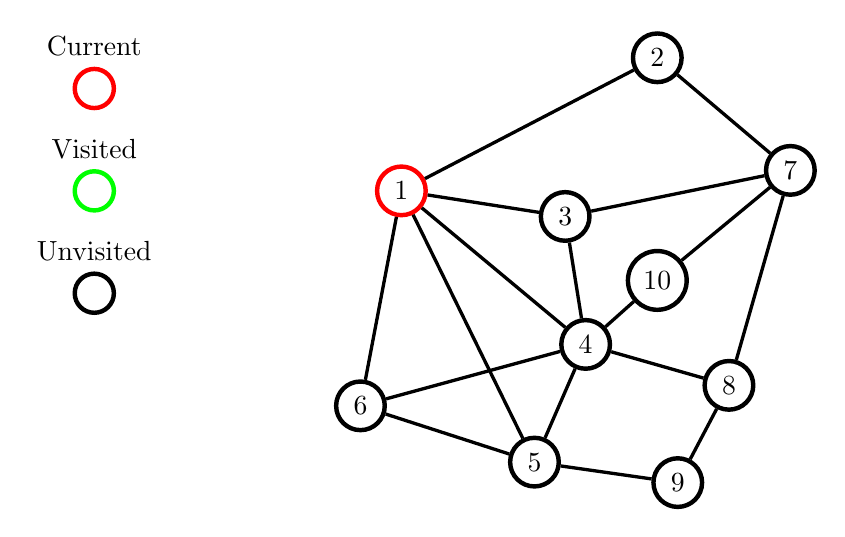
\begin{tikzpicture}[scale=1.3] 
\node[shape=circle, draw=red, 	ultra thick, scale=1.5pt, label={Current}] (U) at (-3, 1) {}; 
\node[shape=circle, draw=green,  ultra thick, scale=1.5pt, label={Visited}] (U) at (-3, 0) {}; 
\node[shape=circle, draw=black, ultra thick, scale=1.5pt, label={Unvisited}] (U) at (-3, -1) {}; 
\node[shape=circle,draw=red, ultra thick] (1) at (0,0) {1}; 
\node[shape=circle,draw=black, ultra thick] (2) at (2.5,1.3) {2}; 
\node[shape=circle,draw=black, ultra thick] (3) at (1.6,-0.25) {3}; 
\node[shape=circle,draw=black, ultra thick] (4) at (1.8,-1.5) {4}; 
\node[shape=circle,draw=black, ultra thick] (5) at (1.3,-2.65) {5}; 
\node[shape=circle,draw=black, ultra thick] (6) at (-0.4,-2.1) {6}; 
\node[shape=circle,draw=black, ultra thick] (7) at (3.8,0.2) {7}; 
\node[shape=circle,draw=black, ultra thick] (8) at (3.2,-1.9) {8}; 
\node[shape=circle,draw=black, ultra thick] (9) at (2.7,-2.85) {9}; 
\node[shape=circle,draw=black, ultra thick] (10) at (2.5,-0.875) {10}; 
\path [-,very thick, draw=black] (2) edge  (1);
\path [-,very thick, draw=black] (3) edge  (1);
\path [-,very thick, draw=black] (4) edge  (1);
\path [-,very thick, draw=black] (5) edge  (1);
\path [-,very thick, draw=black] (6) edge  (1);
\path [-,very thick, draw=black] (7) edge  (2);
\path [-,very thick, draw=black] (7) edge  (3);
\path [-,very thick, draw=black] (4) edge  (3);
\path [-,very thick, draw=black] (5) edge  (4);
\path [-,very thick, draw=black] (6) edge  (4);
\path [-,very thick, draw=black] (8) edge  (4);
\path [-,very thick, draw=black] (10) edge  (4);
\path [-,very thick, draw=black] (6) edge  (5);
\path [-,very thick, draw=black] (9) edge  (5);
\path [-,very thick, draw=black] (8) edge  (7);
\path [-,very thick, draw=black] (10) edge  (7);
\path [-,very thick, draw=black] (9) edge  (8);
\end{tikzpicture} 
\end{figure} 
\end{frame} 
\begin{frame}{DFS : Example}
\begin{figure}
\center
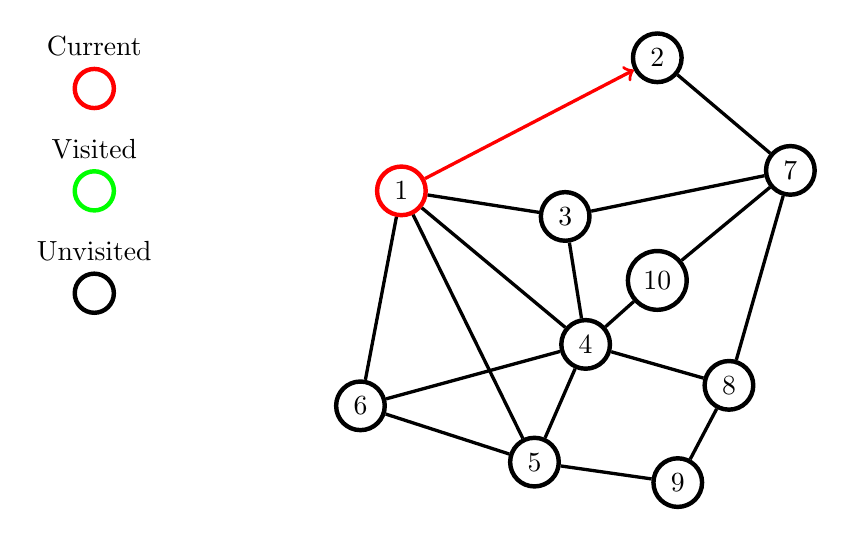
\begin{tikzpicture}[scale=1.3] 
\node[shape=circle, draw=red, 	ultra thick, scale=1.5pt, label={Current}] (U) at (-3, 1) {}; 
\node[shape=circle, draw=green,  ultra thick, scale=1.5pt, label={Visited}] (U) at (-3, 0) {}; 
\node[shape=circle, draw=black, ultra thick, scale=1.5pt, label={Unvisited}] (U) at (-3, -1) {}; 
\node[shape=circle,draw=red, ultra thick] (1) at (0,0) {1}; 
\node[shape=circle,draw=black, ultra thick] (2) at (2.5,1.3) {2}; 
\node[shape=circle,draw=black, ultra thick] (3) at (1.6,-0.25) {3}; 
\node[shape=circle,draw=black, ultra thick] (4) at (1.8,-1.5) {4}; 
\node[shape=circle,draw=black, ultra thick] (5) at (1.3,-2.65) {5}; 
\node[shape=circle,draw=black, ultra thick] (6) at (-0.4,-2.1) {6}; 
\node[shape=circle,draw=black, ultra thick] (7) at (3.8,0.2) {7}; 
\node[shape=circle,draw=black, ultra thick] (8) at (3.2,-1.9) {8}; 
\node[shape=circle,draw=black, ultra thick] (9) at (2.7,-2.85) {9}; 
\node[shape=circle,draw=black, ultra thick] (10) at (2.5,-0.875) {10}; 
\path [-,very thick, draw=black] (3) edge  (1);
\path [-,very thick, draw=black] (4) edge  (1);
\path [-,very thick, draw=black] (5) edge  (1);
\path [-,very thick, draw=black] (6) edge  (1);
\path [-,very thick, draw=black] (7) edge  (2);
\path [-,very thick, draw=black] (7) edge  (3);
\path [-,very thick, draw=black] (4) edge  (3);
\path [-,very thick, draw=black] (5) edge  (4);
\path [-,very thick, draw=black] (6) edge  (4);
\path [-,very thick, draw=black] (8) edge  (4);
\path [-,very thick, draw=black] (10) edge  (4);
\path [-,very thick, draw=black] (6) edge  (5);
\path [-,very thick, draw=black] (9) edge  (5);
\path [-,very thick, draw=black] (8) edge  (7);
\path [-,very thick, draw=black] (10) edge  (7);
\path [-,very thick, draw=black] (9) edge  (8);
\path [->,very thick, draw=red] (1) edge  (2);
\end{tikzpicture} 
\end{figure} 
\end{frame} 
\begin{frame}{DFS : Example}
\begin{figure}
\center
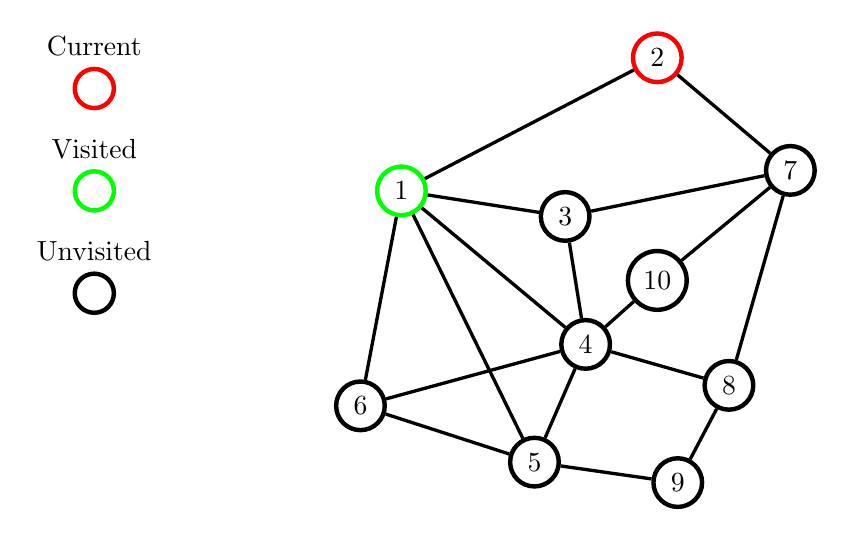
\begin{tikzpicture}[scale=1.3] 
\node[shape=circle, draw=red, 	ultra thick, scale=1.5pt, label={Current}] (U) at (-3, 1) {}; 
\node[shape=circle, draw=green,  ultra thick, scale=1.5pt, label={Visited}] (U) at (-3, 0) {}; 
\node[shape=circle, draw=black, ultra thick, scale=1.5pt, label={Unvisited}] (U) at (-3, -1) {}; 
\node[shape=circle,draw=green, ultra thick] (1) at (0,0) {1}; 
\node[shape=circle,draw=red, ultra thick] (2) at (2.5,1.3) {2}; 
\node[shape=circle,draw=black, ultra thick] (3) at (1.6,-0.25) {3}; 
\node[shape=circle,draw=black, ultra thick] (4) at (1.8,-1.5) {4}; 
\node[shape=circle,draw=black, ultra thick] (5) at (1.3,-2.65) {5}; 
\node[shape=circle,draw=black, ultra thick] (6) at (-0.4,-2.1) {6}; 
\node[shape=circle,draw=black, ultra thick] (7) at (3.8,0.2) {7}; 
\node[shape=circle,draw=black, ultra thick] (8) at (3.2,-1.9) {8}; 
\node[shape=circle,draw=black, ultra thick] (9) at (2.7,-2.85) {9}; 
\node[shape=circle,draw=black, ultra thick] (10) at (2.5,-0.875) {10}; 
\path [-,very thick, draw=black] (2) edge  (1);
\path [-,very thick, draw=black] (3) edge  (1);
\path [-,very thick, draw=black] (4) edge  (1);
\path [-,very thick, draw=black] (5) edge  (1);
\path [-,very thick, draw=black] (6) edge  (1);
\path [-,very thick, draw=black] (7) edge  (2);
\path [-,very thick, draw=black] (7) edge  (3);
\path [-,very thick, draw=black] (4) edge  (3);
\path [-,very thick, draw=black] (5) edge  (4);
\path [-,very thick, draw=black] (6) edge  (4);
\path [-,very thick, draw=black] (8) edge  (4);
\path [-,very thick, draw=black] (10) edge  (4);
\path [-,very thick, draw=black] (6) edge  (5);
\path [-,very thick, draw=black] (9) edge  (5);
\path [-,very thick, draw=black] (8) edge  (7);
\path [-,very thick, draw=black] (10) edge  (7);
\path [-,very thick, draw=black] (9) edge  (8);
\end{tikzpicture} 
\end{figure} 
\end{frame} 
\begin{frame}{DFS : Example}
\begin{figure}
\center
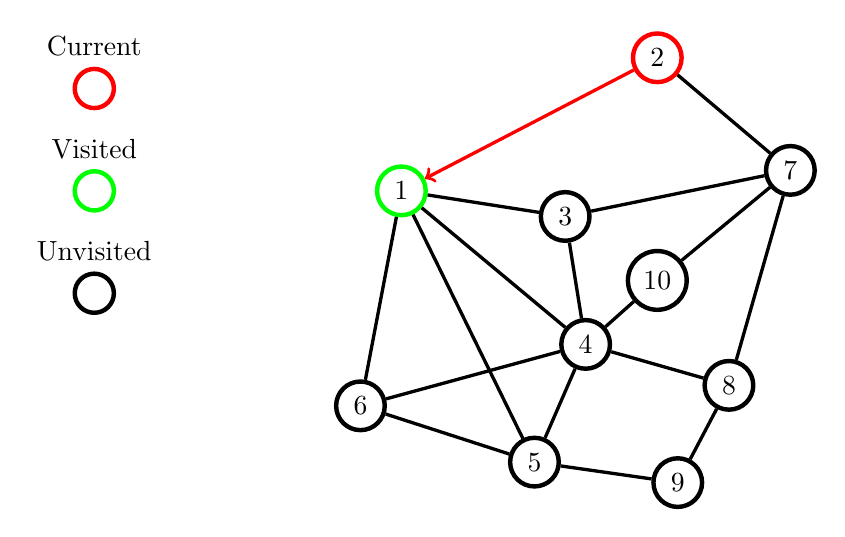
\begin{tikzpicture}[scale=1.3] 
\node[shape=circle, draw=red, 	ultra thick, scale=1.5pt, label={Current}] (U) at (-3, 1) {}; 
\node[shape=circle, draw=green,  ultra thick, scale=1.5pt, label={Visited}] (U) at (-3, 0) {}; 
\node[shape=circle, draw=black, ultra thick, scale=1.5pt, label={Unvisited}] (U) at (-3, -1) {}; 
\node[shape=circle,draw=green, ultra thick] (1) at (0,0) {1}; 
\node[shape=circle,draw=red, ultra thick] (2) at (2.5,1.3) {2}; 
\node[shape=circle,draw=black, ultra thick] (3) at (1.6,-0.25) {3}; 
\node[shape=circle,draw=black, ultra thick] (4) at (1.8,-1.5) {4}; 
\node[shape=circle,draw=black, ultra thick] (5) at (1.3,-2.65) {5}; 
\node[shape=circle,draw=black, ultra thick] (6) at (-0.4,-2.1) {6}; 
\node[shape=circle,draw=black, ultra thick] (7) at (3.8,0.2) {7}; 
\node[shape=circle,draw=black, ultra thick] (8) at (3.2,-1.9) {8}; 
\node[shape=circle,draw=black, ultra thick] (9) at (2.7,-2.85) {9}; 
\node[shape=circle,draw=black, ultra thick] (10) at (2.5,-0.875) {10}; 
\path [-,very thick, draw=black] (3) edge  (1);
\path [-,very thick, draw=black] (4) edge  (1);
\path [-,very thick, draw=black] (5) edge  (1);
\path [-,very thick, draw=black] (6) edge  (1);
\path [-,very thick, draw=black] (7) edge  (2);
\path [-,very thick, draw=black] (7) edge  (3);
\path [-,very thick, draw=black] (4) edge  (3);
\path [-,very thick, draw=black] (5) edge  (4);
\path [-,very thick, draw=black] (6) edge  (4);
\path [-,very thick, draw=black] (8) edge  (4);
\path [-,very thick, draw=black] (10) edge  (4);
\path [-,very thick, draw=black] (6) edge  (5);
\path [-,very thick, draw=black] (9) edge  (5);
\path [-,very thick, draw=black] (8) edge  (7);
\path [-,very thick, draw=black] (10) edge  (7);
\path [-,very thick, draw=black] (9) edge  (8);
\path [->,very thick, draw=red] (2) edge  (1);
\end{tikzpicture} 
\end{figure} 
\end{frame} 
\begin{frame}{DFS : Example}
\begin{figure}
\center
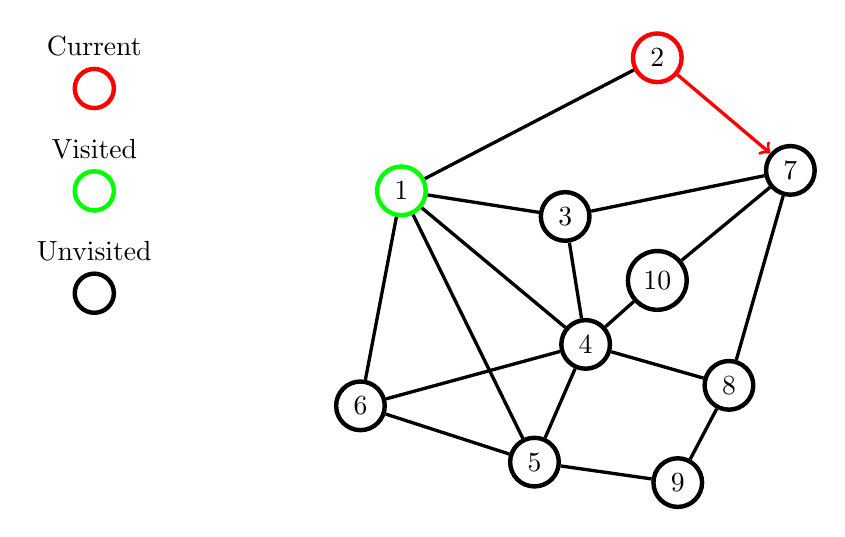
\begin{tikzpicture}[scale=1.3] 
\node[shape=circle, draw=red, 	ultra thick, scale=1.5pt, label={Current}] (U) at (-3, 1) {}; 
\node[shape=circle, draw=green,  ultra thick, scale=1.5pt, label={Visited}] (U) at (-3, 0) {}; 
\node[shape=circle, draw=black, ultra thick, scale=1.5pt, label={Unvisited}] (U) at (-3, -1) {}; 
\node[shape=circle,draw=green, ultra thick] (1) at (0,0) {1}; 
\node[shape=circle,draw=red, ultra thick] (2) at (2.5,1.3) {2}; 
\node[shape=circle,draw=black, ultra thick] (3) at (1.6,-0.25) {3}; 
\node[shape=circle,draw=black, ultra thick] (4) at (1.8,-1.5) {4}; 
\node[shape=circle,draw=black, ultra thick] (5) at (1.3,-2.65) {5}; 
\node[shape=circle,draw=black, ultra thick] (6) at (-0.4,-2.1) {6}; 
\node[shape=circle,draw=black, ultra thick] (7) at (3.8,0.2) {7}; 
\node[shape=circle,draw=black, ultra thick] (8) at (3.2,-1.9) {8}; 
\node[shape=circle,draw=black, ultra thick] (9) at (2.7,-2.85) {9}; 
\node[shape=circle,draw=black, ultra thick] (10) at (2.5,-0.875) {10}; 
\path [-,very thick, draw=black] (2) edge  (1);
\path [-,very thick, draw=black] (3) edge  (1);
\path [-,very thick, draw=black] (4) edge  (1);
\path [-,very thick, draw=black] (5) edge  (1);
\path [-,very thick, draw=black] (6) edge  (1);
\path [-,very thick, draw=black] (7) edge  (3);
\path [-,very thick, draw=black] (4) edge  (3);
\path [-,very thick, draw=black] (5) edge  (4);
\path [-,very thick, draw=black] (6) edge  (4);
\path [-,very thick, draw=black] (8) edge  (4);
\path [-,very thick, draw=black] (10) edge  (4);
\path [-,very thick, draw=black] (6) edge  (5);
\path [-,very thick, draw=black] (9) edge  (5);
\path [-,very thick, draw=black] (8) edge  (7);
\path [-,very thick, draw=black] (10) edge  (7);
\path [-,very thick, draw=black] (9) edge  (8);
\path [->,very thick, draw=red] (2) edge  (7);
\end{tikzpicture} 
\end{figure} 
\end{frame} 
\begin{frame}{DFS : Example}
\begin{figure}
\center
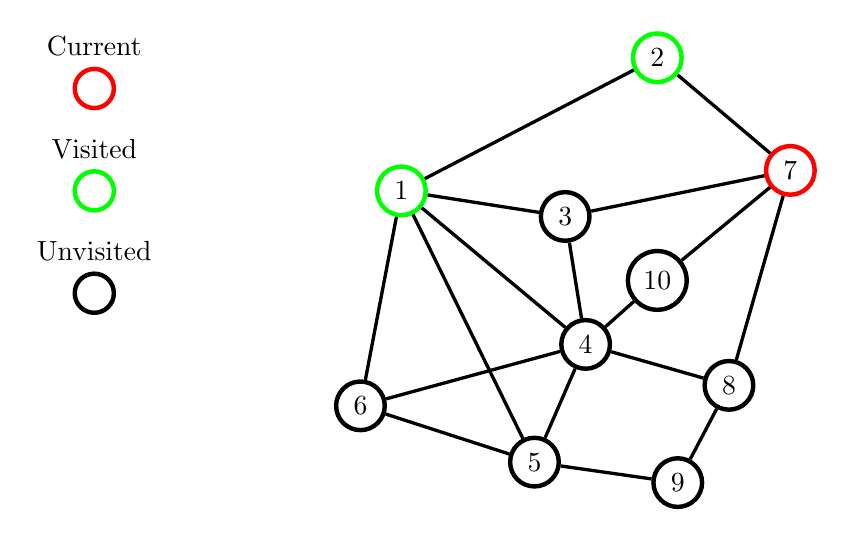
\begin{tikzpicture}[scale=1.3] 
\node[shape=circle, draw=red, 	ultra thick, scale=1.5pt, label={Current}] (U) at (-3, 1) {}; 
\node[shape=circle, draw=green,  ultra thick, scale=1.5pt, label={Visited}] (U) at (-3, 0) {}; 
\node[shape=circle, draw=black, ultra thick, scale=1.5pt, label={Unvisited}] (U) at (-3, -1) {}; 
\node[shape=circle,draw=green, ultra thick] (1) at (0,0) {1}; 
\node[shape=circle,draw=green, ultra thick] (2) at (2.5,1.3) {2}; 
\node[shape=circle,draw=black, ultra thick] (3) at (1.6,-0.25) {3}; 
\node[shape=circle,draw=black, ultra thick] (4) at (1.8,-1.5) {4}; 
\node[shape=circle,draw=black, ultra thick] (5) at (1.3,-2.65) {5}; 
\node[shape=circle,draw=black, ultra thick] (6) at (-0.4,-2.1) {6}; 
\node[shape=circle,draw=red, ultra thick] (7) at (3.8,0.2) {7}; 
\node[shape=circle,draw=black, ultra thick] (8) at (3.2,-1.9) {8}; 
\node[shape=circle,draw=black, ultra thick] (9) at (2.7,-2.85) {9}; 
\node[shape=circle,draw=black, ultra thick] (10) at (2.5,-0.875) {10}; 
\path [-,very thick, draw=black] (2) edge  (1);
\path [-,very thick, draw=black] (3) edge  (1);
\path [-,very thick, draw=black] (4) edge  (1);
\path [-,very thick, draw=black] (5) edge  (1);
\path [-,very thick, draw=black] (6) edge  (1);
\path [-,very thick, draw=black] (7) edge  (2);
\path [-,very thick, draw=black] (7) edge  (3);
\path [-,very thick, draw=black] (4) edge  (3);
\path [-,very thick, draw=black] (5) edge  (4);
\path [-,very thick, draw=black] (6) edge  (4);
\path [-,very thick, draw=black] (8) edge  (4);
\path [-,very thick, draw=black] (10) edge  (4);
\path [-,very thick, draw=black] (6) edge  (5);
\path [-,very thick, draw=black] (9) edge  (5);
\path [-,very thick, draw=black] (8) edge  (7);
\path [-,very thick, draw=black] (10) edge  (7);
\path [-,very thick, draw=black] (9) edge  (8);
\end{tikzpicture} 
\end{figure} 
\end{frame} 
\begin{frame}{DFS : Example}
\begin{figure}
\center
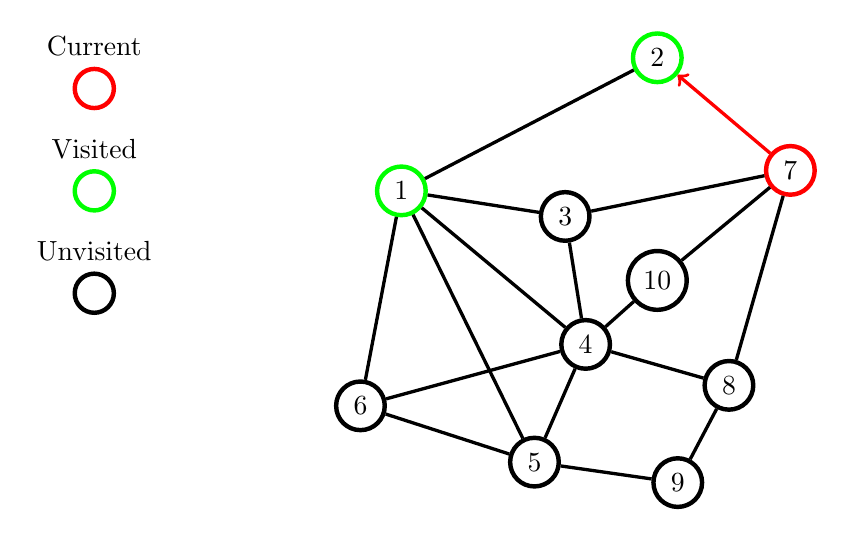
\begin{tikzpicture}[scale=1.3] 
\node[shape=circle, draw=red, 	ultra thick, scale=1.5pt, label={Current}] (U) at (-3, 1) {}; 
\node[shape=circle, draw=green,  ultra thick, scale=1.5pt, label={Visited}] (U) at (-3, 0) {}; 
\node[shape=circle, draw=black, ultra thick, scale=1.5pt, label={Unvisited}] (U) at (-3, -1) {}; 
\node[shape=circle,draw=green, ultra thick] (1) at (0,0) {1}; 
\node[shape=circle,draw=green, ultra thick] (2) at (2.5,1.3) {2}; 
\node[shape=circle,draw=black, ultra thick] (3) at (1.6,-0.25) {3}; 
\node[shape=circle,draw=black, ultra thick] (4) at (1.8,-1.5) {4}; 
\node[shape=circle,draw=black, ultra thick] (5) at (1.3,-2.65) {5}; 
\node[shape=circle,draw=black, ultra thick] (6) at (-0.4,-2.1) {6}; 
\node[shape=circle,draw=red, ultra thick] (7) at (3.8,0.2) {7}; 
\node[shape=circle,draw=black, ultra thick] (8) at (3.2,-1.9) {8}; 
\node[shape=circle,draw=black, ultra thick] (9) at (2.7,-2.85) {9}; 
\node[shape=circle,draw=black, ultra thick] (10) at (2.5,-0.875) {10}; 
\path [-,very thick, draw=black] (2) edge  (1);
\path [-,very thick, draw=black] (3) edge  (1);
\path [-,very thick, draw=black] (4) edge  (1);
\path [-,very thick, draw=black] (5) edge  (1);
\path [-,very thick, draw=black] (6) edge  (1);
\path [-,very thick, draw=black] (7) edge  (3);
\path [-,very thick, draw=black] (4) edge  (3);
\path [-,very thick, draw=black] (5) edge  (4);
\path [-,very thick, draw=black] (6) edge  (4);
\path [-,very thick, draw=black] (8) edge  (4);
\path [-,very thick, draw=black] (10) edge  (4);
\path [-,very thick, draw=black] (6) edge  (5);
\path [-,very thick, draw=black] (9) edge  (5);
\path [-,very thick, draw=black] (8) edge  (7);
\path [-,very thick, draw=black] (10) edge  (7);
\path [-,very thick, draw=black] (9) edge  (8);
\path [->,very thick, draw=red] (7) edge  (2);
\end{tikzpicture} 
\end{figure} 
\end{frame} 
\begin{frame}{DFS : Example}
\begin{figure}
\center
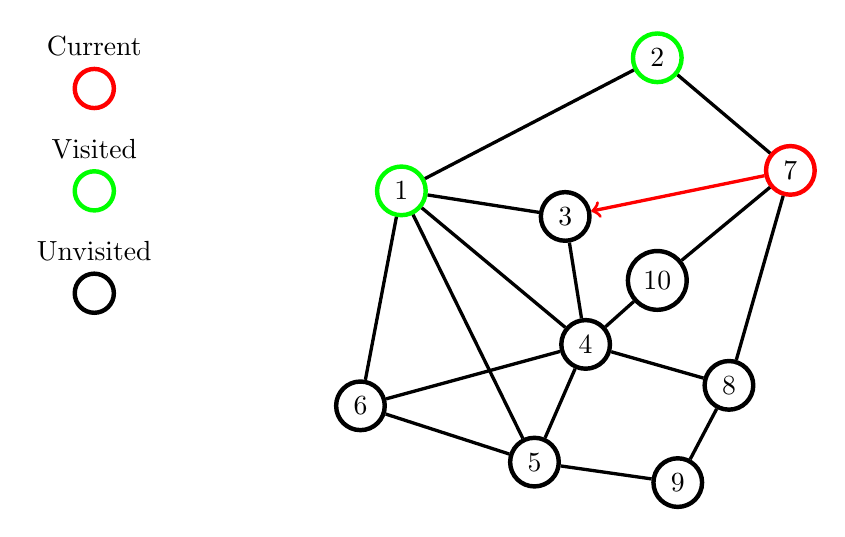
\begin{tikzpicture}[scale=1.3] 
\node[shape=circle, draw=red, 	ultra thick, scale=1.5pt, label={Current}] (U) at (-3, 1) {}; 
\node[shape=circle, draw=green,  ultra thick, scale=1.5pt, label={Visited}] (U) at (-3, 0) {}; 
\node[shape=circle, draw=black, ultra thick, scale=1.5pt, label={Unvisited}] (U) at (-3, -1) {}; 
\node[shape=circle,draw=green, ultra thick] (1) at (0,0) {1}; 
\node[shape=circle,draw=green, ultra thick] (2) at (2.5,1.3) {2}; 
\node[shape=circle,draw=black, ultra thick] (3) at (1.6,-0.25) {3}; 
\node[shape=circle,draw=black, ultra thick] (4) at (1.8,-1.5) {4}; 
\node[shape=circle,draw=black, ultra thick] (5) at (1.3,-2.65) {5}; 
\node[shape=circle,draw=black, ultra thick] (6) at (-0.4,-2.1) {6}; 
\node[shape=circle,draw=red, ultra thick] (7) at (3.8,0.2) {7}; 
\node[shape=circle,draw=black, ultra thick] (8) at (3.2,-1.9) {8}; 
\node[shape=circle,draw=black, ultra thick] (9) at (2.7,-2.85) {9}; 
\node[shape=circle,draw=black, ultra thick] (10) at (2.5,-0.875) {10}; 
\path [-,very thick, draw=black] (2) edge  (1);
\path [-,very thick, draw=black] (3) edge  (1);
\path [-,very thick, draw=black] (4) edge  (1);
\path [-,very thick, draw=black] (5) edge  (1);
\path [-,very thick, draw=black] (6) edge  (1);
\path [-,very thick, draw=black] (7) edge  (2);
\path [-,very thick, draw=black] (4) edge  (3);
\path [-,very thick, draw=black] (5) edge  (4);
\path [-,very thick, draw=black] (6) edge  (4);
\path [-,very thick, draw=black] (8) edge  (4);
\path [-,very thick, draw=black] (10) edge  (4);
\path [-,very thick, draw=black] (6) edge  (5);
\path [-,very thick, draw=black] (9) edge  (5);
\path [-,very thick, draw=black] (8) edge  (7);
\path [-,very thick, draw=black] (10) edge  (7);
\path [-,very thick, draw=black] (9) edge  (8);
\path [->,very thick, draw=red] (7) edge  (3);
\end{tikzpicture} 
\end{figure} 
\end{frame} 
\begin{frame}{DFS : Example}
\begin{figure}
\center
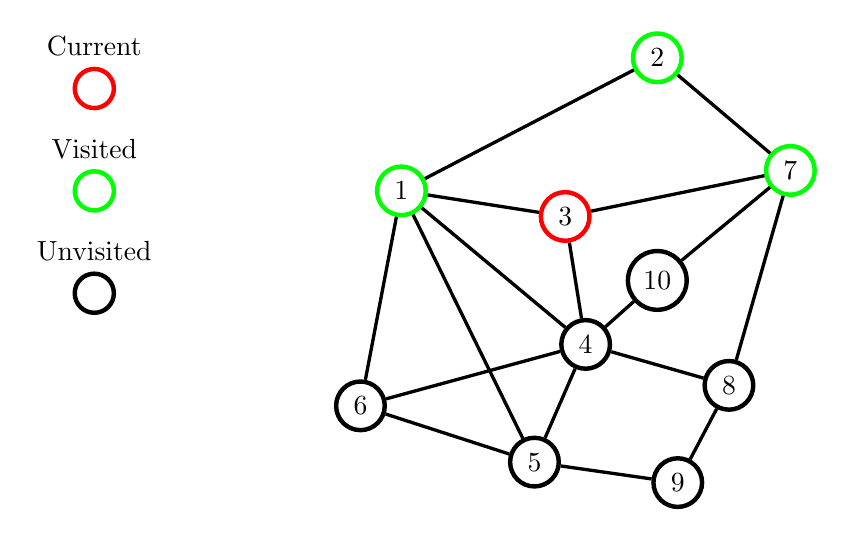
\begin{tikzpicture}[scale=1.3] 
\node[shape=circle, draw=red, 	ultra thick, scale=1.5pt, label={Current}] (U) at (-3, 1) {}; 
\node[shape=circle, draw=green,  ultra thick, scale=1.5pt, label={Visited}] (U) at (-3, 0) {}; 
\node[shape=circle, draw=black, ultra thick, scale=1.5pt, label={Unvisited}] (U) at (-3, -1) {}; 
\node[shape=circle,draw=green, ultra thick] (1) at (0,0) {1}; 
\node[shape=circle,draw=green, ultra thick] (2) at (2.5,1.3) {2}; 
\node[shape=circle,draw=red, ultra thick] (3) at (1.6,-0.25) {3}; 
\node[shape=circle,draw=black, ultra thick] (4) at (1.8,-1.5) {4}; 
\node[shape=circle,draw=black, ultra thick] (5) at (1.3,-2.65) {5}; 
\node[shape=circle,draw=black, ultra thick] (6) at (-0.4,-2.1) {6}; 
\node[shape=circle,draw=green, ultra thick] (7) at (3.8,0.2) {7}; 
\node[shape=circle,draw=black, ultra thick] (8) at (3.2,-1.9) {8}; 
\node[shape=circle,draw=black, ultra thick] (9) at (2.7,-2.85) {9}; 
\node[shape=circle,draw=black, ultra thick] (10) at (2.5,-0.875) {10}; 
\path [-,very thick, draw=black] (2) edge  (1);
\path [-,very thick, draw=black] (3) edge  (1);
\path [-,very thick, draw=black] (4) edge  (1);
\path [-,very thick, draw=black] (5) edge  (1);
\path [-,very thick, draw=black] (6) edge  (1);
\path [-,very thick, draw=black] (7) edge  (2);
\path [-,very thick, draw=black] (7) edge  (3);
\path [-,very thick, draw=black] (4) edge  (3);
\path [-,very thick, draw=black] (5) edge  (4);
\path [-,very thick, draw=black] (6) edge  (4);
\path [-,very thick, draw=black] (8) edge  (4);
\path [-,very thick, draw=black] (10) edge  (4);
\path [-,very thick, draw=black] (6) edge  (5);
\path [-,very thick, draw=black] (9) edge  (5);
\path [-,very thick, draw=black] (8) edge  (7);
\path [-,very thick, draw=black] (10) edge  (7);
\path [-,very thick, draw=black] (9) edge  (8);
\end{tikzpicture} 
\end{figure} 
\end{frame} 
\begin{frame}{DFS : Example}
\begin{figure}
\center
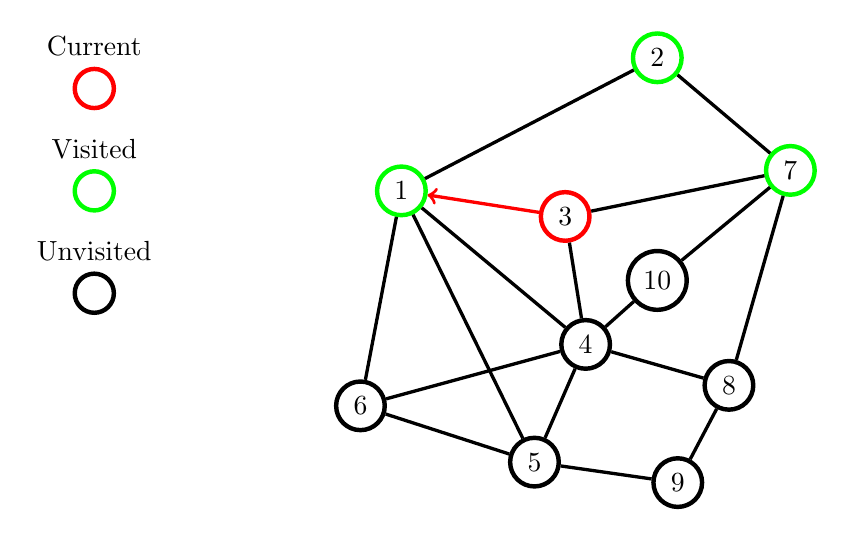
\begin{tikzpicture}[scale=1.3] 
\node[shape=circle, draw=red, 	ultra thick, scale=1.5pt, label={Current}] (U) at (-3, 1) {}; 
\node[shape=circle, draw=green,  ultra thick, scale=1.5pt, label={Visited}] (U) at (-3, 0) {}; 
\node[shape=circle, draw=black, ultra thick, scale=1.5pt, label={Unvisited}] (U) at (-3, -1) {}; 
\node[shape=circle,draw=green, ultra thick] (1) at (0,0) {1}; 
\node[shape=circle,draw=green, ultra thick] (2) at (2.5,1.3) {2}; 
\node[shape=circle,draw=red, ultra thick] (3) at (1.6,-0.25) {3}; 
\node[shape=circle,draw=black, ultra thick] (4) at (1.8,-1.5) {4}; 
\node[shape=circle,draw=black, ultra thick] (5) at (1.3,-2.65) {5}; 
\node[shape=circle,draw=black, ultra thick] (6) at (-0.4,-2.1) {6}; 
\node[shape=circle,draw=green, ultra thick] (7) at (3.8,0.2) {7}; 
\node[shape=circle,draw=black, ultra thick] (8) at (3.2,-1.9) {8}; 
\node[shape=circle,draw=black, ultra thick] (9) at (2.7,-2.85) {9}; 
\node[shape=circle,draw=black, ultra thick] (10) at (2.5,-0.875) {10}; 
\path [-,very thick, draw=black] (2) edge  (1);
\path [-,very thick, draw=black] (4) edge  (1);
\path [-,very thick, draw=black] (5) edge  (1);
\path [-,very thick, draw=black] (6) edge  (1);
\path [-,very thick, draw=black] (7) edge  (2);
\path [-,very thick, draw=black] (7) edge  (3);
\path [-,very thick, draw=black] (4) edge  (3);
\path [-,very thick, draw=black] (5) edge  (4);
\path [-,very thick, draw=black] (6) edge  (4);
\path [-,very thick, draw=black] (8) edge  (4);
\path [-,very thick, draw=black] (10) edge  (4);
\path [-,very thick, draw=black] (6) edge  (5);
\path [-,very thick, draw=black] (9) edge  (5);
\path [-,very thick, draw=black] (8) edge  (7);
\path [-,very thick, draw=black] (10) edge  (7);
\path [-,very thick, draw=black] (9) edge  (8);
\path [->,very thick, draw=red] (3) edge  (1);
\end{tikzpicture} 
\end{figure} 
\end{frame} 
\begin{frame}{DFS : Example}
\begin{figure}
\center
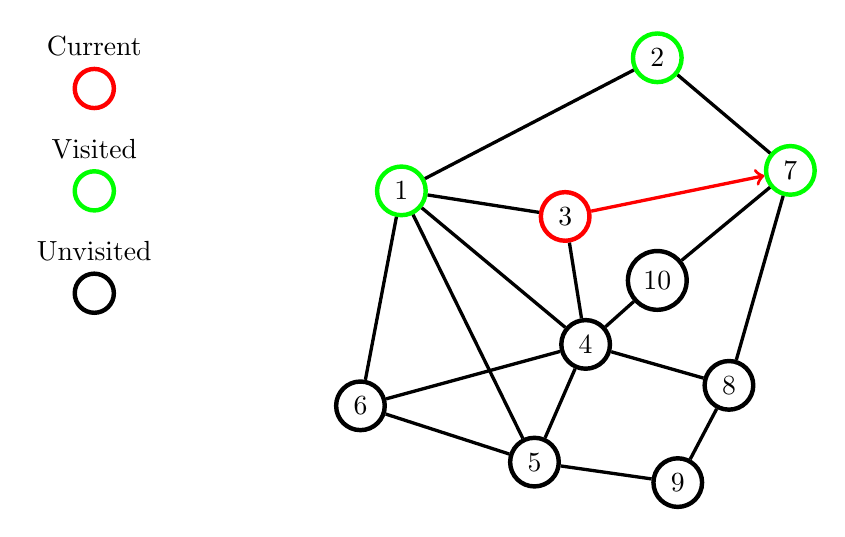
\begin{tikzpicture}[scale=1.3] 
\node[shape=circle, draw=red, 	ultra thick, scale=1.5pt, label={Current}] (U) at (-3, 1) {}; 
\node[shape=circle, draw=green,  ultra thick, scale=1.5pt, label={Visited}] (U) at (-3, 0) {}; 
\node[shape=circle, draw=black, ultra thick, scale=1.5pt, label={Unvisited}] (U) at (-3, -1) {}; 
\node[shape=circle,draw=green, ultra thick] (1) at (0,0) {1}; 
\node[shape=circle,draw=green, ultra thick] (2) at (2.5,1.3) {2}; 
\node[shape=circle,draw=red, ultra thick] (3) at (1.6,-0.25) {3}; 
\node[shape=circle,draw=black, ultra thick] (4) at (1.8,-1.5) {4}; 
\node[shape=circle,draw=black, ultra thick] (5) at (1.3,-2.65) {5}; 
\node[shape=circle,draw=black, ultra thick] (6) at (-0.4,-2.1) {6}; 
\node[shape=circle,draw=green, ultra thick] (7) at (3.8,0.2) {7}; 
\node[shape=circle,draw=black, ultra thick] (8) at (3.2,-1.9) {8}; 
\node[shape=circle,draw=black, ultra thick] (9) at (2.7,-2.85) {9}; 
\node[shape=circle,draw=black, ultra thick] (10) at (2.5,-0.875) {10}; 
\path [-,very thick, draw=black] (2) edge  (1);
\path [-,very thick, draw=black] (3) edge  (1);
\path [-,very thick, draw=black] (4) edge  (1);
\path [-,very thick, draw=black] (5) edge  (1);
\path [-,very thick, draw=black] (6) edge  (1);
\path [-,very thick, draw=black] (7) edge  (2);
\path [-,very thick, draw=black] (4) edge  (3);
\path [-,very thick, draw=black] (5) edge  (4);
\path [-,very thick, draw=black] (6) edge  (4);
\path [-,very thick, draw=black] (8) edge  (4);
\path [-,very thick, draw=black] (10) edge  (4);
\path [-,very thick, draw=black] (6) edge  (5);
\path [-,very thick, draw=black] (9) edge  (5);
\path [-,very thick, draw=black] (8) edge  (7);
\path [-,very thick, draw=black] (10) edge  (7);
\path [-,very thick, draw=black] (9) edge  (8);
\path [->,very thick, draw=red] (3) edge  (7);
\end{tikzpicture} 
\end{figure} 
\end{frame} 
\begin{frame}{DFS : Example}
\begin{figure}
\center
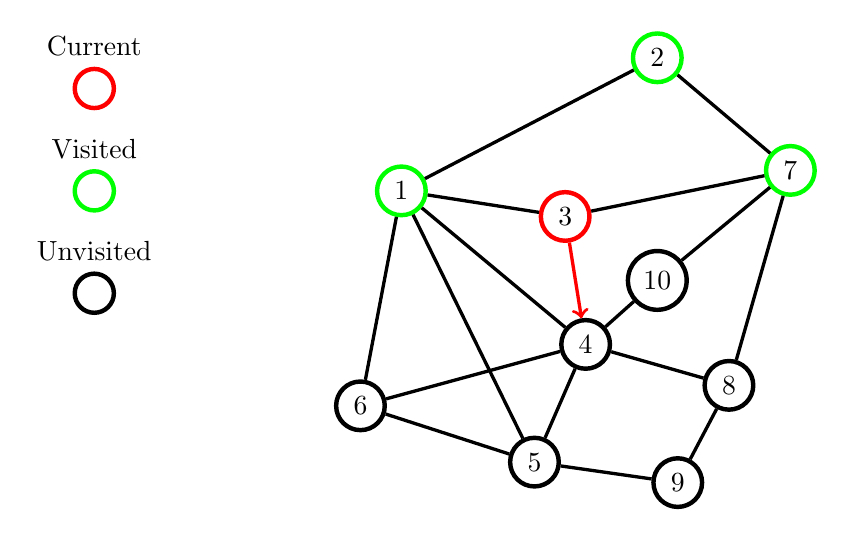
\begin{tikzpicture}[scale=1.3] 
\node[shape=circle, draw=red, 	ultra thick, scale=1.5pt, label={Current}] (U) at (-3, 1) {}; 
\node[shape=circle, draw=green,  ultra thick, scale=1.5pt, label={Visited}] (U) at (-3, 0) {}; 
\node[shape=circle, draw=black, ultra thick, scale=1.5pt, label={Unvisited}] (U) at (-3, -1) {}; 
\node[shape=circle,draw=green, ultra thick] (1) at (0,0) {1}; 
\node[shape=circle,draw=green, ultra thick] (2) at (2.5,1.3) {2}; 
\node[shape=circle,draw=red, ultra thick] (3) at (1.6,-0.25) {3}; 
\node[shape=circle,draw=black, ultra thick] (4) at (1.8,-1.5) {4}; 
\node[shape=circle,draw=black, ultra thick] (5) at (1.3,-2.65) {5}; 
\node[shape=circle,draw=black, ultra thick] (6) at (-0.4,-2.1) {6}; 
\node[shape=circle,draw=green, ultra thick] (7) at (3.8,0.2) {7}; 
\node[shape=circle,draw=black, ultra thick] (8) at (3.2,-1.9) {8}; 
\node[shape=circle,draw=black, ultra thick] (9) at (2.7,-2.85) {9}; 
\node[shape=circle,draw=black, ultra thick] (10) at (2.5,-0.875) {10}; 
\path [-,very thick, draw=black] (2) edge  (1);
\path [-,very thick, draw=black] (3) edge  (1);
\path [-,very thick, draw=black] (4) edge  (1);
\path [-,very thick, draw=black] (5) edge  (1);
\path [-,very thick, draw=black] (6) edge  (1);
\path [-,very thick, draw=black] (7) edge  (2);
\path [-,very thick, draw=black] (7) edge  (3);
\path [-,very thick, draw=black] (5) edge  (4);
\path [-,very thick, draw=black] (6) edge  (4);
\path [-,very thick, draw=black] (8) edge  (4);
\path [-,very thick, draw=black] (10) edge  (4);
\path [-,very thick, draw=black] (6) edge  (5);
\path [-,very thick, draw=black] (9) edge  (5);
\path [-,very thick, draw=black] (8) edge  (7);
\path [-,very thick, draw=black] (10) edge  (7);
\path [-,very thick, draw=black] (9) edge  (8);
\path [->,very thick, draw=red] (3) edge  (4);
\end{tikzpicture} 
\end{figure} 
\end{frame} 
\begin{frame}{DFS : Example}
\begin{figure}
\center
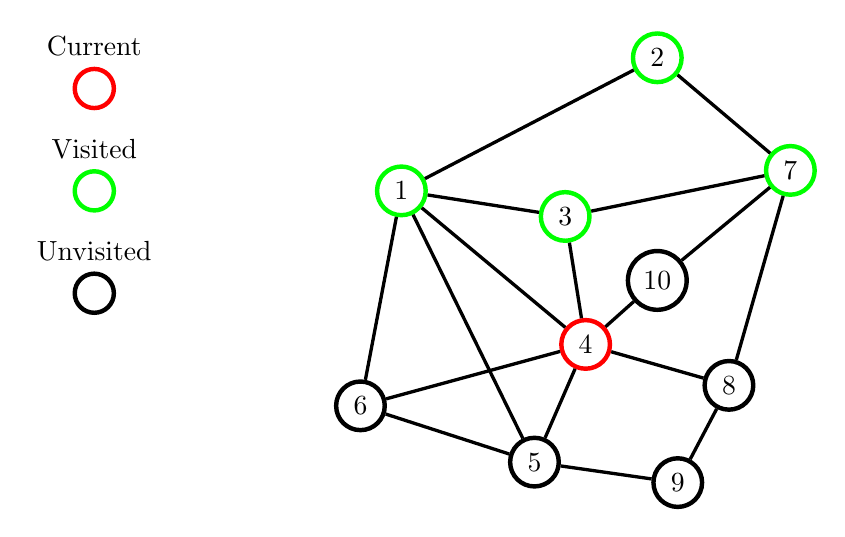
\begin{tikzpicture}[scale=1.3] 
\node[shape=circle, draw=red, 	ultra thick, scale=1.5pt, label={Current}] (U) at (-3, 1) {}; 
\node[shape=circle, draw=green,  ultra thick, scale=1.5pt, label={Visited}] (U) at (-3, 0) {}; 
\node[shape=circle, draw=black, ultra thick, scale=1.5pt, label={Unvisited}] (U) at (-3, -1) {}; 
\node[shape=circle,draw=green, ultra thick] (1) at (0,0) {1}; 
\node[shape=circle,draw=green, ultra thick] (2) at (2.5,1.3) {2}; 
\node[shape=circle,draw=green, ultra thick] (3) at (1.6,-0.25) {3}; 
\node[shape=circle,draw=red, ultra thick] (4) at (1.8,-1.5) {4}; 
\node[shape=circle,draw=black, ultra thick] (5) at (1.3,-2.65) {5}; 
\node[shape=circle,draw=black, ultra thick] (6) at (-0.4,-2.1) {6}; 
\node[shape=circle,draw=green, ultra thick] (7) at (3.8,0.2) {7}; 
\node[shape=circle,draw=black, ultra thick] (8) at (3.2,-1.9) {8}; 
\node[shape=circle,draw=black, ultra thick] (9) at (2.7,-2.85) {9}; 
\node[shape=circle,draw=black, ultra thick] (10) at (2.5,-0.875) {10}; 
\path [-,very thick, draw=black] (2) edge  (1);
\path [-,very thick, draw=black] (3) edge  (1);
\path [-,very thick, draw=black] (4) edge  (1);
\path [-,very thick, draw=black] (5) edge  (1);
\path [-,very thick, draw=black] (6) edge  (1);
\path [-,very thick, draw=black] (7) edge  (2);
\path [-,very thick, draw=black] (7) edge  (3);
\path [-,very thick, draw=black] (4) edge  (3);
\path [-,very thick, draw=black] (5) edge  (4);
\path [-,very thick, draw=black] (6) edge  (4);
\path [-,very thick, draw=black] (8) edge  (4);
\path [-,very thick, draw=black] (10) edge  (4);
\path [-,very thick, draw=black] (6) edge  (5);
\path [-,very thick, draw=black] (9) edge  (5);
\path [-,very thick, draw=black] (8) edge  (7);
\path [-,very thick, draw=black] (10) edge  (7);
\path [-,very thick, draw=black] (9) edge  (8);
\end{tikzpicture} 
\end{figure} 
\end{frame} 
\begin{frame}{DFS : Example}
\begin{figure}
\center
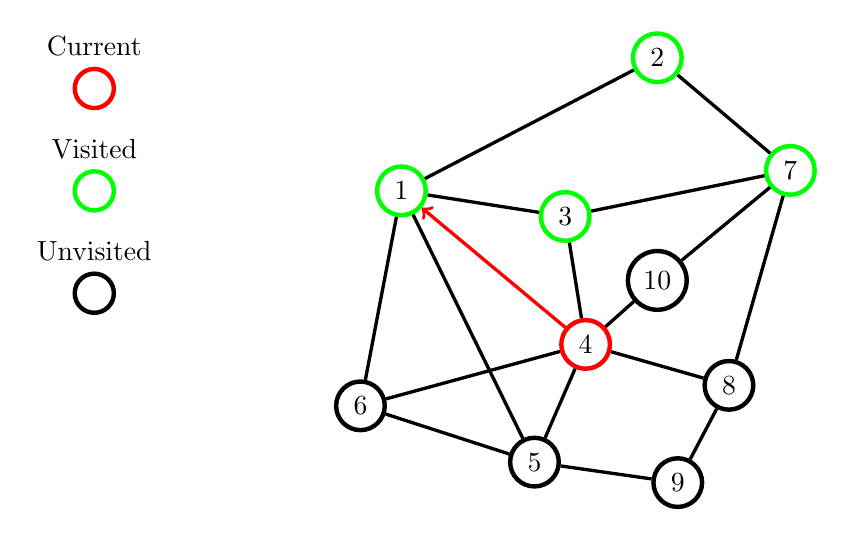
\begin{tikzpicture}[scale=1.3] 
\node[shape=circle, draw=red, 	ultra thick, scale=1.5pt, label={Current}] (U) at (-3, 1) {}; 
\node[shape=circle, draw=green,  ultra thick, scale=1.5pt, label={Visited}] (U) at (-3, 0) {}; 
\node[shape=circle, draw=black, ultra thick, scale=1.5pt, label={Unvisited}] (U) at (-3, -1) {}; 
\node[shape=circle,draw=green, ultra thick] (1) at (0,0) {1}; 
\node[shape=circle,draw=green, ultra thick] (2) at (2.5,1.3) {2}; 
\node[shape=circle,draw=green, ultra thick] (3) at (1.6,-0.25) {3}; 
\node[shape=circle,draw=red, ultra thick] (4) at (1.8,-1.5) {4}; 
\node[shape=circle,draw=black, ultra thick] (5) at (1.3,-2.65) {5}; 
\node[shape=circle,draw=black, ultra thick] (6) at (-0.4,-2.1) {6}; 
\node[shape=circle,draw=green, ultra thick] (7) at (3.8,0.2) {7}; 
\node[shape=circle,draw=black, ultra thick] (8) at (3.2,-1.9) {8}; 
\node[shape=circle,draw=black, ultra thick] (9) at (2.7,-2.85) {9}; 
\node[shape=circle,draw=black, ultra thick] (10) at (2.5,-0.875) {10}; 
\path [-,very thick, draw=black] (2) edge  (1);
\path [-,very thick, draw=black] (3) edge  (1);
\path [-,very thick, draw=black] (5) edge  (1);
\path [-,very thick, draw=black] (6) edge  (1);
\path [-,very thick, draw=black] (7) edge  (2);
\path [-,very thick, draw=black] (7) edge  (3);
\path [-,very thick, draw=black] (4) edge  (3);
\path [-,very thick, draw=black] (5) edge  (4);
\path [-,very thick, draw=black] (6) edge  (4);
\path [-,very thick, draw=black] (8) edge  (4);
\path [-,very thick, draw=black] (10) edge  (4);
\path [-,very thick, draw=black] (6) edge  (5);
\path [-,very thick, draw=black] (9) edge  (5);
\path [-,very thick, draw=black] (8) edge  (7);
\path [-,very thick, draw=black] (10) edge  (7);
\path [-,very thick, draw=black] (9) edge  (8);
\path [->,very thick, draw=red] (4) edge  (1);
\end{tikzpicture} 
\end{figure} 
\end{frame} 
\begin{frame}{DFS : Example}
\begin{figure}
\center
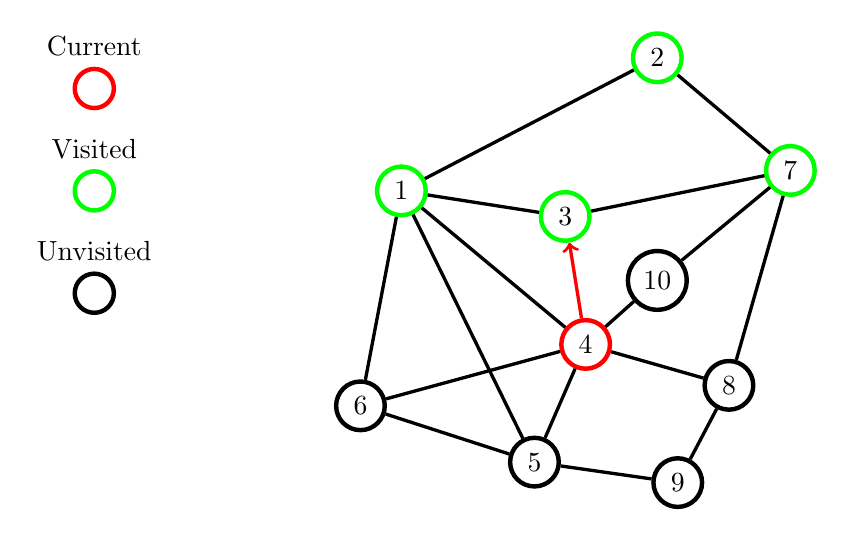
\begin{tikzpicture}[scale=1.3] 
\node[shape=circle, draw=red, 	ultra thick, scale=1.5pt, label={Current}] (U) at (-3, 1) {}; 
\node[shape=circle, draw=green,  ultra thick, scale=1.5pt, label={Visited}] (U) at (-3, 0) {}; 
\node[shape=circle, draw=black, ultra thick, scale=1.5pt, label={Unvisited}] (U) at (-3, -1) {}; 
\node[shape=circle,draw=green, ultra thick] (1) at (0,0) {1}; 
\node[shape=circle,draw=green, ultra thick] (2) at (2.5,1.3) {2}; 
\node[shape=circle,draw=green, ultra thick] (3) at (1.6,-0.25) {3}; 
\node[shape=circle,draw=red, ultra thick] (4) at (1.8,-1.5) {4}; 
\node[shape=circle,draw=black, ultra thick] (5) at (1.3,-2.65) {5}; 
\node[shape=circle,draw=black, ultra thick] (6) at (-0.4,-2.1) {6}; 
\node[shape=circle,draw=green, ultra thick] (7) at (3.8,0.2) {7}; 
\node[shape=circle,draw=black, ultra thick] (8) at (3.2,-1.9) {8}; 
\node[shape=circle,draw=black, ultra thick] (9) at (2.7,-2.85) {9}; 
\node[shape=circle,draw=black, ultra thick] (10) at (2.5,-0.875) {10}; 
\path [-,very thick, draw=black] (2) edge  (1);
\path [-,very thick, draw=black] (3) edge  (1);
\path [-,very thick, draw=black] (4) edge  (1);
\path [-,very thick, draw=black] (5) edge  (1);
\path [-,very thick, draw=black] (6) edge  (1);
\path [-,very thick, draw=black] (7) edge  (2);
\path [-,very thick, draw=black] (7) edge  (3);
\path [-,very thick, draw=black] (5) edge  (4);
\path [-,very thick, draw=black] (6) edge  (4);
\path [-,very thick, draw=black] (8) edge  (4);
\path [-,very thick, draw=black] (10) edge  (4);
\path [-,very thick, draw=black] (6) edge  (5);
\path [-,very thick, draw=black] (9) edge  (5);
\path [-,very thick, draw=black] (8) edge  (7);
\path [-,very thick, draw=black] (10) edge  (7);
\path [-,very thick, draw=black] (9) edge  (8);
\path [->,very thick, draw=red] (4) edge  (3);
\end{tikzpicture} 
\end{figure} 
\end{frame} 
\begin{frame}{DFS : Example}
\begin{figure}
\center
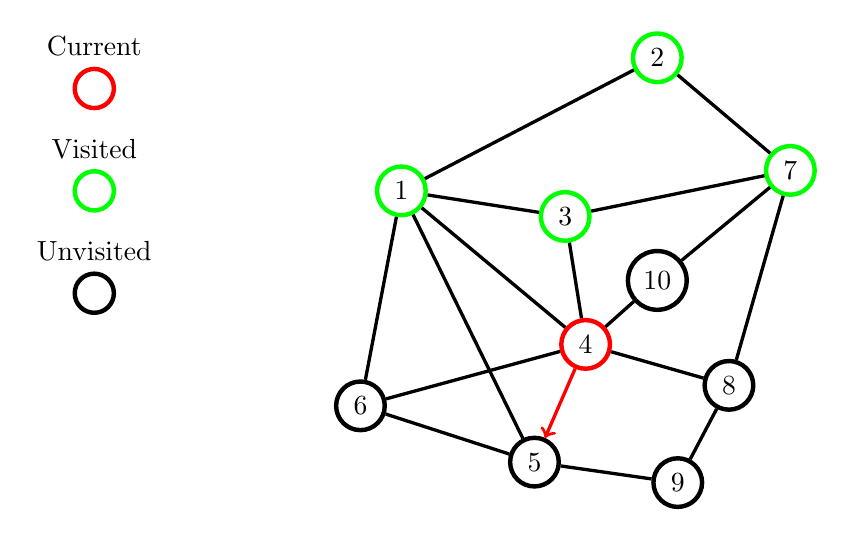
\begin{tikzpicture}[scale=1.3] 
\node[shape=circle, draw=red, 	ultra thick, scale=1.5pt, label={Current}] (U) at (-3, 1) {}; 
\node[shape=circle, draw=green,  ultra thick, scale=1.5pt, label={Visited}] (U) at (-3, 0) {}; 
\node[shape=circle, draw=black, ultra thick, scale=1.5pt, label={Unvisited}] (U) at (-3, -1) {}; 
\node[shape=circle,draw=green, ultra thick] (1) at (0,0) {1}; 
\node[shape=circle,draw=green, ultra thick] (2) at (2.5,1.3) {2}; 
\node[shape=circle,draw=green, ultra thick] (3) at (1.6,-0.25) {3}; 
\node[shape=circle,draw=red, ultra thick] (4) at (1.8,-1.5) {4}; 
\node[shape=circle,draw=black, ultra thick] (5) at (1.3,-2.65) {5}; 
\node[shape=circle,draw=black, ultra thick] (6) at (-0.4,-2.1) {6}; 
\node[shape=circle,draw=green, ultra thick] (7) at (3.8,0.2) {7}; 
\node[shape=circle,draw=black, ultra thick] (8) at (3.2,-1.9) {8}; 
\node[shape=circle,draw=black, ultra thick] (9) at (2.7,-2.85) {9}; 
\node[shape=circle,draw=black, ultra thick] (10) at (2.5,-0.875) {10}; 
\path [-,very thick, draw=black] (2) edge  (1);
\path [-,very thick, draw=black] (3) edge  (1);
\path [-,very thick, draw=black] (4) edge  (1);
\path [-,very thick, draw=black] (5) edge  (1);
\path [-,very thick, draw=black] (6) edge  (1);
\path [-,very thick, draw=black] (7) edge  (2);
\path [-,very thick, draw=black] (7) edge  (3);
\path [-,very thick, draw=black] (4) edge  (3);
\path [-,very thick, draw=black] (6) edge  (4);
\path [-,very thick, draw=black] (8) edge  (4);
\path [-,very thick, draw=black] (10) edge  (4);
\path [-,very thick, draw=black] (6) edge  (5);
\path [-,very thick, draw=black] (9) edge  (5);
\path [-,very thick, draw=black] (8) edge  (7);
\path [-,very thick, draw=black] (10) edge  (7);
\path [-,very thick, draw=black] (9) edge  (8);
\path [->,very thick, draw=red] (4) edge  (5);
\end{tikzpicture} 
\end{figure} 
\end{frame} 
\begin{frame}{DFS : Example}
\begin{figure}
\center
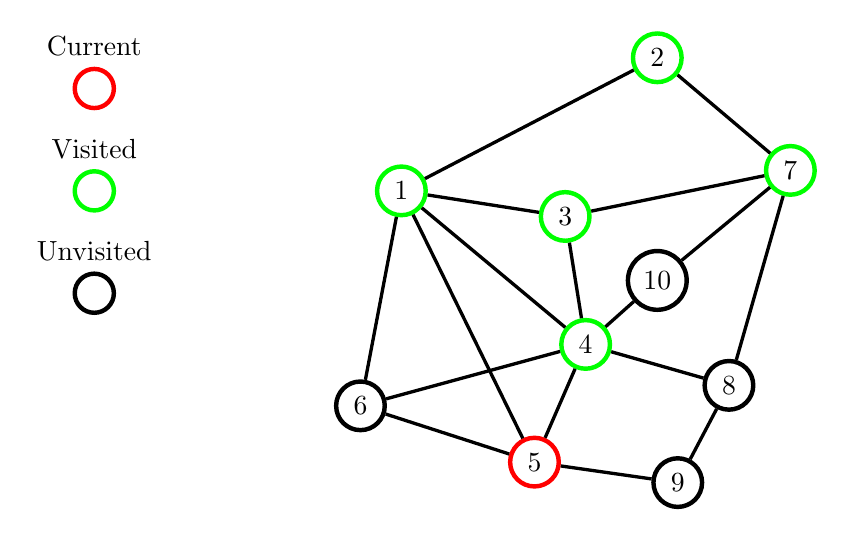
\begin{tikzpicture}[scale=1.3] 
\node[shape=circle, draw=red, 	ultra thick, scale=1.5pt, label={Current}] (U) at (-3, 1) {}; 
\node[shape=circle, draw=green,  ultra thick, scale=1.5pt, label={Visited}] (U) at (-3, 0) {}; 
\node[shape=circle, draw=black, ultra thick, scale=1.5pt, label={Unvisited}] (U) at (-3, -1) {}; 
\node[shape=circle,draw=green, ultra thick] (1) at (0,0) {1}; 
\node[shape=circle,draw=green, ultra thick] (2) at (2.5,1.3) {2}; 
\node[shape=circle,draw=green, ultra thick] (3) at (1.6,-0.25) {3}; 
\node[shape=circle,draw=green, ultra thick] (4) at (1.8,-1.5) {4}; 
\node[shape=circle,draw=red, ultra thick] (5) at (1.3,-2.65) {5}; 
\node[shape=circle,draw=black, ultra thick] (6) at (-0.4,-2.1) {6}; 
\node[shape=circle,draw=green, ultra thick] (7) at (3.8,0.2) {7}; 
\node[shape=circle,draw=black, ultra thick] (8) at (3.2,-1.9) {8}; 
\node[shape=circle,draw=black, ultra thick] (9) at (2.7,-2.85) {9}; 
\node[shape=circle,draw=black, ultra thick] (10) at (2.5,-0.875) {10}; 
\path [-,very thick, draw=black] (2) edge  (1);
\path [-,very thick, draw=black] (3) edge  (1);
\path [-,very thick, draw=black] (4) edge  (1);
\path [-,very thick, draw=black] (5) edge  (1);
\path [-,very thick, draw=black] (6) edge  (1);
\path [-,very thick, draw=black] (7) edge  (2);
\path [-,very thick, draw=black] (7) edge  (3);
\path [-,very thick, draw=black] (4) edge  (3);
\path [-,very thick, draw=black] (5) edge  (4);
\path [-,very thick, draw=black] (6) edge  (4);
\path [-,very thick, draw=black] (8) edge  (4);
\path [-,very thick, draw=black] (10) edge  (4);
\path [-,very thick, draw=black] (6) edge  (5);
\path [-,very thick, draw=black] (9) edge  (5);
\path [-,very thick, draw=black] (8) edge  (7);
\path [-,very thick, draw=black] (10) edge  (7);
\path [-,very thick, draw=black] (9) edge  (8);
\end{tikzpicture} 
\end{figure} 
\end{frame} 
\begin{frame}{DFS : Example}
\begin{figure}
\center
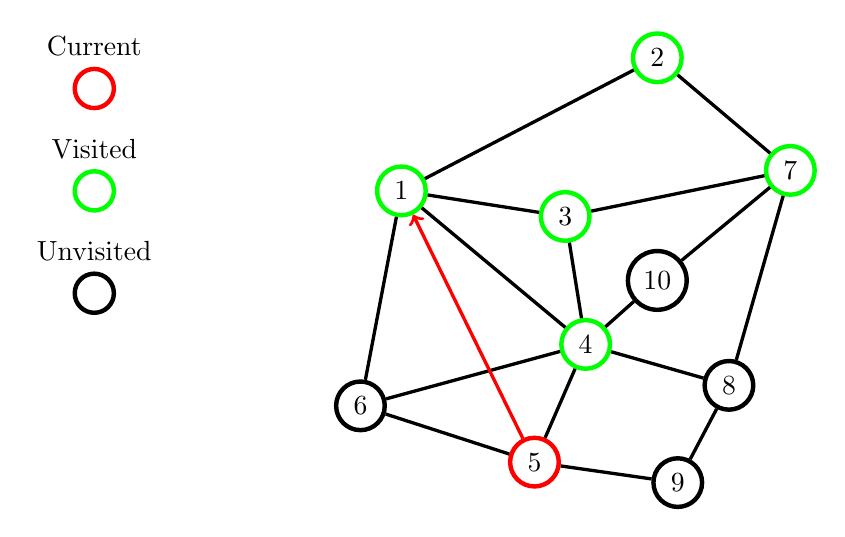
\begin{tikzpicture}[scale=1.3] 
\node[shape=circle, draw=red, 	ultra thick, scale=1.5pt, label={Current}] (U) at (-3, 1) {}; 
\node[shape=circle, draw=green,  ultra thick, scale=1.5pt, label={Visited}] (U) at (-3, 0) {}; 
\node[shape=circle, draw=black, ultra thick, scale=1.5pt, label={Unvisited}] (U) at (-3, -1) {}; 
\node[shape=circle,draw=green, ultra thick] (1) at (0,0) {1}; 
\node[shape=circle,draw=green, ultra thick] (2) at (2.5,1.3) {2}; 
\node[shape=circle,draw=green, ultra thick] (3) at (1.6,-0.25) {3}; 
\node[shape=circle,draw=green, ultra thick] (4) at (1.8,-1.5) {4}; 
\node[shape=circle,draw=red, ultra thick] (5) at (1.3,-2.65) {5}; 
\node[shape=circle,draw=black, ultra thick] (6) at (-0.4,-2.1) {6}; 
\node[shape=circle,draw=green, ultra thick] (7) at (3.8,0.2) {7}; 
\node[shape=circle,draw=black, ultra thick] (8) at (3.2,-1.9) {8}; 
\node[shape=circle,draw=black, ultra thick] (9) at (2.7,-2.85) {9}; 
\node[shape=circle,draw=black, ultra thick] (10) at (2.5,-0.875) {10}; 
\path [-,very thick, draw=black] (2) edge  (1);
\path [-,very thick, draw=black] (3) edge  (1);
\path [-,very thick, draw=black] (4) edge  (1);
\path [-,very thick, draw=black] (6) edge  (1);
\path [-,very thick, draw=black] (7) edge  (2);
\path [-,very thick, draw=black] (7) edge  (3);
\path [-,very thick, draw=black] (4) edge  (3);
\path [-,very thick, draw=black] (5) edge  (4);
\path [-,very thick, draw=black] (6) edge  (4);
\path [-,very thick, draw=black] (8) edge  (4);
\path [-,very thick, draw=black] (10) edge  (4);
\path [-,very thick, draw=black] (6) edge  (5);
\path [-,very thick, draw=black] (9) edge  (5);
\path [-,very thick, draw=black] (8) edge  (7);
\path [-,very thick, draw=black] (10) edge  (7);
\path [-,very thick, draw=black] (9) edge  (8);
\path [->,very thick, draw=red] (5) edge  (1);
\end{tikzpicture} 
\end{figure} 
\end{frame} 
\begin{frame}{DFS : Example}
\begin{figure}
\center
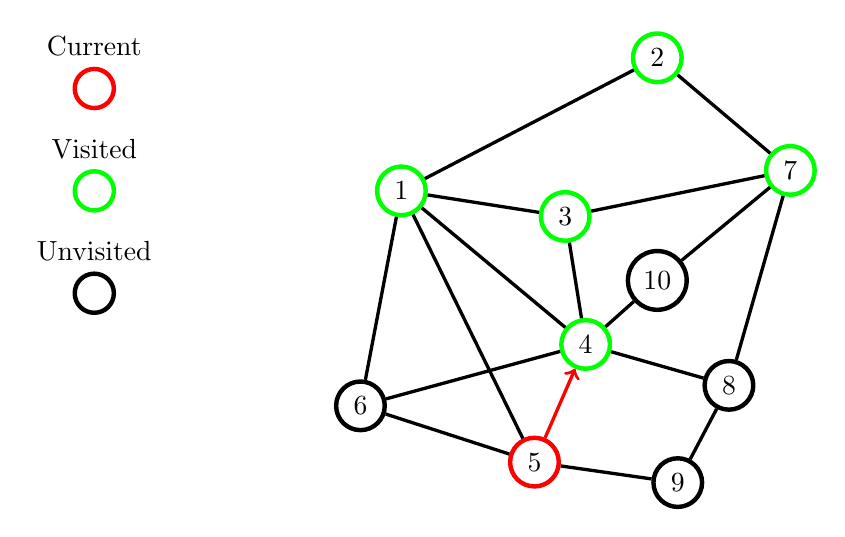
\begin{tikzpicture}[scale=1.3] 
\node[shape=circle, draw=red, 	ultra thick, scale=1.5pt, label={Current}] (U) at (-3, 1) {}; 
\node[shape=circle, draw=green,  ultra thick, scale=1.5pt, label={Visited}] (U) at (-3, 0) {}; 
\node[shape=circle, draw=black, ultra thick, scale=1.5pt, label={Unvisited}] (U) at (-3, -1) {}; 
\node[shape=circle,draw=green, ultra thick] (1) at (0,0) {1}; 
\node[shape=circle,draw=green, ultra thick] (2) at (2.5,1.3) {2}; 
\node[shape=circle,draw=green, ultra thick] (3) at (1.6,-0.25) {3}; 
\node[shape=circle,draw=green, ultra thick] (4) at (1.8,-1.5) {4}; 
\node[shape=circle,draw=red, ultra thick] (5) at (1.3,-2.65) {5}; 
\node[shape=circle,draw=black, ultra thick] (6) at (-0.4,-2.1) {6}; 
\node[shape=circle,draw=green, ultra thick] (7) at (3.8,0.2) {7}; 
\node[shape=circle,draw=black, ultra thick] (8) at (3.2,-1.9) {8}; 
\node[shape=circle,draw=black, ultra thick] (9) at (2.7,-2.85) {9}; 
\node[shape=circle,draw=black, ultra thick] (10) at (2.5,-0.875) {10}; 
\path [-,very thick, draw=black] (2) edge  (1);
\path [-,very thick, draw=black] (3) edge  (1);
\path [-,very thick, draw=black] (4) edge  (1);
\path [-,very thick, draw=black] (5) edge  (1);
\path [-,very thick, draw=black] (6) edge  (1);
\path [-,very thick, draw=black] (7) edge  (2);
\path [-,very thick, draw=black] (7) edge  (3);
\path [-,very thick, draw=black] (4) edge  (3);
\path [-,very thick, draw=black] (6) edge  (4);
\path [-,very thick, draw=black] (8) edge  (4);
\path [-,very thick, draw=black] (10) edge  (4);
\path [-,very thick, draw=black] (6) edge  (5);
\path [-,very thick, draw=black] (9) edge  (5);
\path [-,very thick, draw=black] (8) edge  (7);
\path [-,very thick, draw=black] (10) edge  (7);
\path [-,very thick, draw=black] (9) edge  (8);
\path [->,very thick, draw=red] (5) edge  (4);
\end{tikzpicture} 
\end{figure} 
\end{frame} 
\begin{frame}{DFS : Example}
\begin{figure}
\center
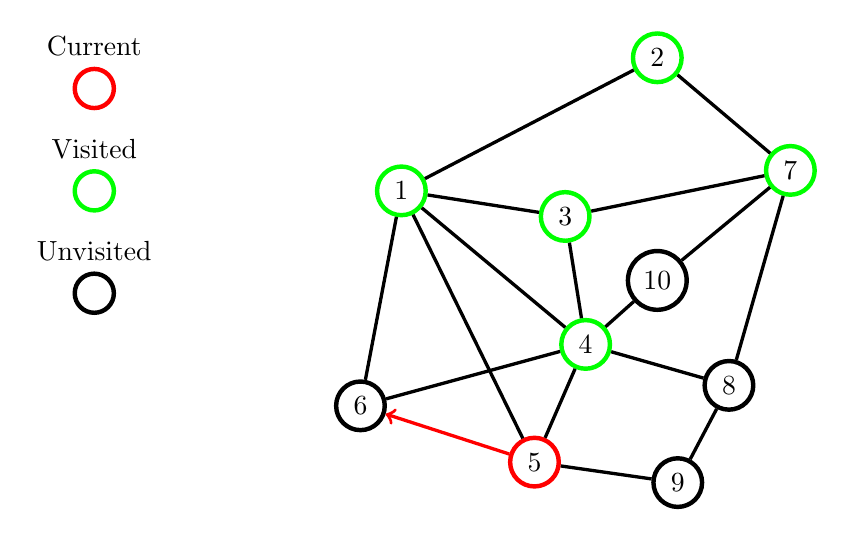
\begin{tikzpicture}[scale=1.3] 
\node[shape=circle, draw=red, 	ultra thick, scale=1.5pt, label={Current}] (U) at (-3, 1) {}; 
\node[shape=circle, draw=green,  ultra thick, scale=1.5pt, label={Visited}] (U) at (-3, 0) {}; 
\node[shape=circle, draw=black, ultra thick, scale=1.5pt, label={Unvisited}] (U) at (-3, -1) {}; 
\node[shape=circle,draw=green, ultra thick] (1) at (0,0) {1}; 
\node[shape=circle,draw=green, ultra thick] (2) at (2.5,1.3) {2}; 
\node[shape=circle,draw=green, ultra thick] (3) at (1.6,-0.25) {3}; 
\node[shape=circle,draw=green, ultra thick] (4) at (1.8,-1.5) {4}; 
\node[shape=circle,draw=red, ultra thick] (5) at (1.3,-2.65) {5}; 
\node[shape=circle,draw=black, ultra thick] (6) at (-0.4,-2.1) {6}; 
\node[shape=circle,draw=green, ultra thick] (7) at (3.8,0.2) {7}; 
\node[shape=circle,draw=black, ultra thick] (8) at (3.2,-1.9) {8}; 
\node[shape=circle,draw=black, ultra thick] (9) at (2.7,-2.85) {9}; 
\node[shape=circle,draw=black, ultra thick] (10) at (2.5,-0.875) {10}; 
\path [-,very thick, draw=black] (2) edge  (1);
\path [-,very thick, draw=black] (3) edge  (1);
\path [-,very thick, draw=black] (4) edge  (1);
\path [-,very thick, draw=black] (5) edge  (1);
\path [-,very thick, draw=black] (6) edge  (1);
\path [-,very thick, draw=black] (7) edge  (2);
\path [-,very thick, draw=black] (7) edge  (3);
\path [-,very thick, draw=black] (4) edge  (3);
\path [-,very thick, draw=black] (5) edge  (4);
\path [-,very thick, draw=black] (6) edge  (4);
\path [-,very thick, draw=black] (8) edge  (4);
\path [-,very thick, draw=black] (10) edge  (4);
\path [-,very thick, draw=black] (9) edge  (5);
\path [-,very thick, draw=black] (8) edge  (7);
\path [-,very thick, draw=black] (10) edge  (7);
\path [-,very thick, draw=black] (9) edge  (8);
\path [->,very thick, draw=red] (5) edge  (6);
\end{tikzpicture} 
\end{figure} 
\end{frame} 
\begin{frame}{DFS : Example}
\begin{figure}
\center
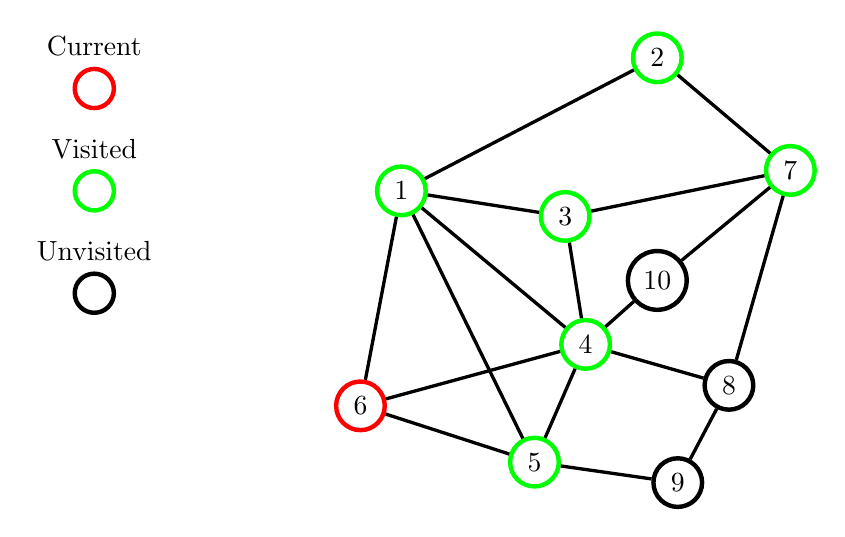
\begin{tikzpicture}[scale=1.3] 
\node[shape=circle, draw=red, 	ultra thick, scale=1.5pt, label={Current}] (U) at (-3, 1) {}; 
\node[shape=circle, draw=green,  ultra thick, scale=1.5pt, label={Visited}] (U) at (-3, 0) {}; 
\node[shape=circle, draw=black, ultra thick, scale=1.5pt, label={Unvisited}] (U) at (-3, -1) {}; 
\node[shape=circle,draw=green, ultra thick] (1) at (0,0) {1}; 
\node[shape=circle,draw=green, ultra thick] (2) at (2.5,1.3) {2}; 
\node[shape=circle,draw=green, ultra thick] (3) at (1.6,-0.25) {3}; 
\node[shape=circle,draw=green, ultra thick] (4) at (1.8,-1.5) {4}; 
\node[shape=circle,draw=green, ultra thick] (5) at (1.3,-2.65) {5}; 
\node[shape=circle,draw=red, ultra thick] (6) at (-0.4,-2.1) {6}; 
\node[shape=circle,draw=green, ultra thick] (7) at (3.8,0.2) {7}; 
\node[shape=circle,draw=black, ultra thick] (8) at (3.2,-1.9) {8}; 
\node[shape=circle,draw=black, ultra thick] (9) at (2.7,-2.85) {9}; 
\node[shape=circle,draw=black, ultra thick] (10) at (2.5,-0.875) {10}; 
\path [-,very thick, draw=black] (2) edge  (1);
\path [-,very thick, draw=black] (3) edge  (1);
\path [-,very thick, draw=black] (4) edge  (1);
\path [-,very thick, draw=black] (5) edge  (1);
\path [-,very thick, draw=black] (6) edge  (1);
\path [-,very thick, draw=black] (7) edge  (2);
\path [-,very thick, draw=black] (7) edge  (3);
\path [-,very thick, draw=black] (4) edge  (3);
\path [-,very thick, draw=black] (5) edge  (4);
\path [-,very thick, draw=black] (6) edge  (4);
\path [-,very thick, draw=black] (8) edge  (4);
\path [-,very thick, draw=black] (10) edge  (4);
\path [-,very thick, draw=black] (6) edge  (5);
\path [-,very thick, draw=black] (9) edge  (5);
\path [-,very thick, draw=black] (8) edge  (7);
\path [-,very thick, draw=black] (10) edge  (7);
\path [-,very thick, draw=black] (9) edge  (8);
\end{tikzpicture} 
\end{figure} 
\end{frame} 
\begin{frame}{DFS : Example}
\begin{figure}
\center
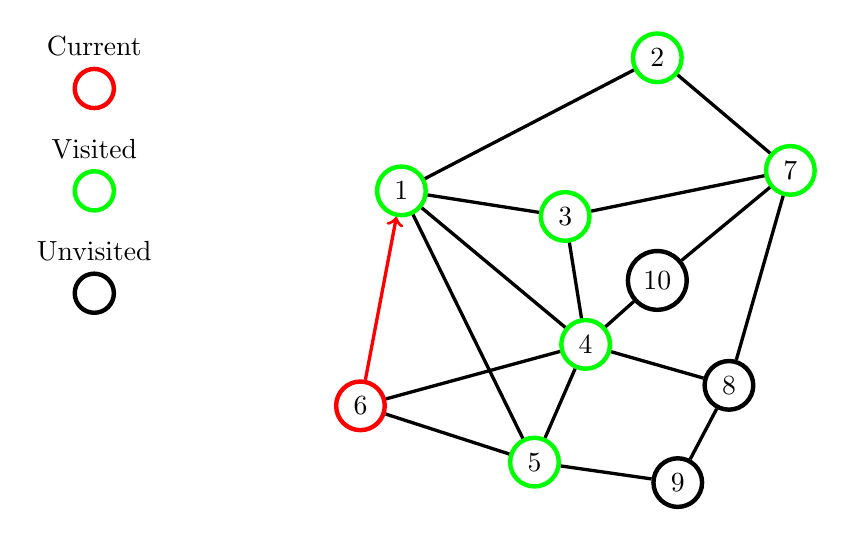
\begin{tikzpicture}[scale=1.3] 
\node[shape=circle, draw=red, 	ultra thick, scale=1.5pt, label={Current}] (U) at (-3, 1) {}; 
\node[shape=circle, draw=green,  ultra thick, scale=1.5pt, label={Visited}] (U) at (-3, 0) {}; 
\node[shape=circle, draw=black, ultra thick, scale=1.5pt, label={Unvisited}] (U) at (-3, -1) {}; 
\node[shape=circle,draw=green, ultra thick] (1) at (0,0) {1}; 
\node[shape=circle,draw=green, ultra thick] (2) at (2.5,1.3) {2}; 
\node[shape=circle,draw=green, ultra thick] (3) at (1.6,-0.25) {3}; 
\node[shape=circle,draw=green, ultra thick] (4) at (1.8,-1.5) {4}; 
\node[shape=circle,draw=green, ultra thick] (5) at (1.3,-2.65) {5}; 
\node[shape=circle,draw=red, ultra thick] (6) at (-0.4,-2.1) {6}; 
\node[shape=circle,draw=green, ultra thick] (7) at (3.8,0.2) {7}; 
\node[shape=circle,draw=black, ultra thick] (8) at (3.2,-1.9) {8}; 
\node[shape=circle,draw=black, ultra thick] (9) at (2.7,-2.85) {9}; 
\node[shape=circle,draw=black, ultra thick] (10) at (2.5,-0.875) {10}; 
\path [-,very thick, draw=black] (2) edge  (1);
\path [-,very thick, draw=black] (3) edge  (1);
\path [-,very thick, draw=black] (4) edge  (1);
\path [-,very thick, draw=black] (5) edge  (1);
\path [-,very thick, draw=black] (7) edge  (2);
\path [-,very thick, draw=black] (7) edge  (3);
\path [-,very thick, draw=black] (4) edge  (3);
\path [-,very thick, draw=black] (5) edge  (4);
\path [-,very thick, draw=black] (6) edge  (4);
\path [-,very thick, draw=black] (8) edge  (4);
\path [-,very thick, draw=black] (10) edge  (4);
\path [-,very thick, draw=black] (6) edge  (5);
\path [-,very thick, draw=black] (9) edge  (5);
\path [-,very thick, draw=black] (8) edge  (7);
\path [-,very thick, draw=black] (10) edge  (7);
\path [-,very thick, draw=black] (9) edge  (8);
\path [->,very thick, draw=red] (6) edge  (1);
\end{tikzpicture} 
\end{figure} 
\end{frame} 
\begin{frame}{DFS : Example}
\begin{figure}
\center
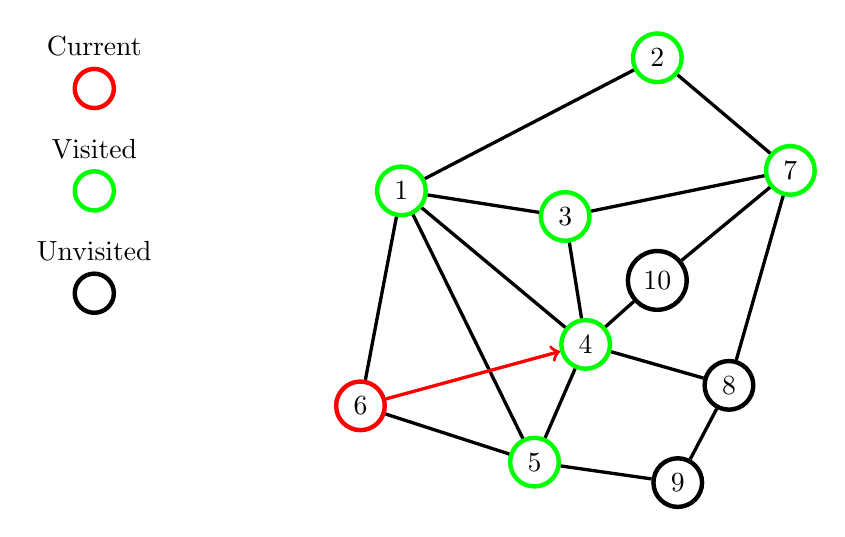
\begin{tikzpicture}[scale=1.3] 
\node[shape=circle, draw=red, 	ultra thick, scale=1.5pt, label={Current}] (U) at (-3, 1) {}; 
\node[shape=circle, draw=green,  ultra thick, scale=1.5pt, label={Visited}] (U) at (-3, 0) {}; 
\node[shape=circle, draw=black, ultra thick, scale=1.5pt, label={Unvisited}] (U) at (-3, -1) {}; 
\node[shape=circle,draw=green, ultra thick] (1) at (0,0) {1}; 
\node[shape=circle,draw=green, ultra thick] (2) at (2.5,1.3) {2}; 
\node[shape=circle,draw=green, ultra thick] (3) at (1.6,-0.25) {3}; 
\node[shape=circle,draw=green, ultra thick] (4) at (1.8,-1.5) {4}; 
\node[shape=circle,draw=green, ultra thick] (5) at (1.3,-2.65) {5}; 
\node[shape=circle,draw=red, ultra thick] (6) at (-0.4,-2.1) {6}; 
\node[shape=circle,draw=green, ultra thick] (7) at (3.8,0.2) {7}; 
\node[shape=circle,draw=black, ultra thick] (8) at (3.2,-1.9) {8}; 
\node[shape=circle,draw=black, ultra thick] (9) at (2.7,-2.85) {9}; 
\node[shape=circle,draw=black, ultra thick] (10) at (2.5,-0.875) {10}; 
\path [-,very thick, draw=black] (2) edge  (1);
\path [-,very thick, draw=black] (3) edge  (1);
\path [-,very thick, draw=black] (4) edge  (1);
\path [-,very thick, draw=black] (5) edge  (1);
\path [-,very thick, draw=black] (6) edge  (1);
\path [-,very thick, draw=black] (7) edge  (2);
\path [-,very thick, draw=black] (7) edge  (3);
\path [-,very thick, draw=black] (4) edge  (3);
\path [-,very thick, draw=black] (5) edge  (4);
\path [-,very thick, draw=black] (8) edge  (4);
\path [-,very thick, draw=black] (10) edge  (4);
\path [-,very thick, draw=black] (6) edge  (5);
\path [-,very thick, draw=black] (9) edge  (5);
\path [-,very thick, draw=black] (8) edge  (7);
\path [-,very thick, draw=black] (10) edge  (7);
\path [-,very thick, draw=black] (9) edge  (8);
\path [->,very thick, draw=red] (6) edge  (4);
\end{tikzpicture} 
\end{figure} 
\end{frame} 
\begin{frame}{DFS : Example}
\begin{figure}
\center
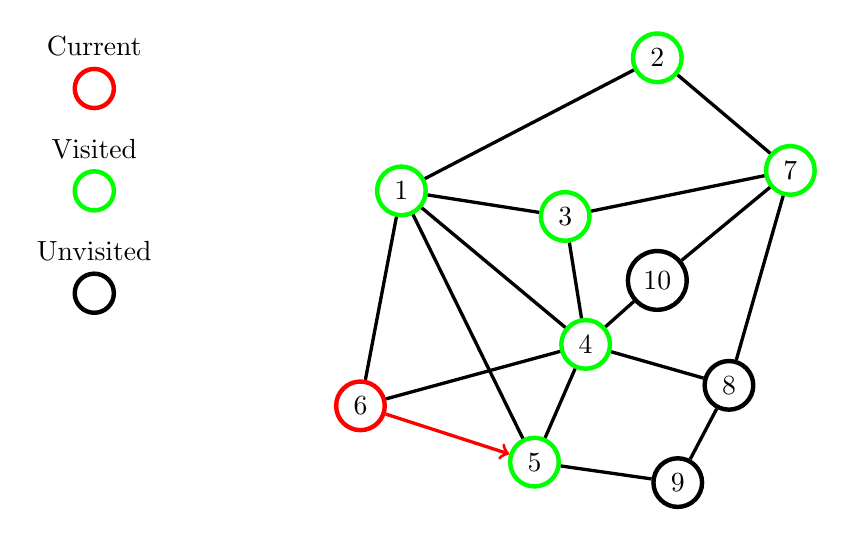
\begin{tikzpicture}[scale=1.3] 
\node[shape=circle, draw=red, 	ultra thick, scale=1.5pt, label={Current}] (U) at (-3, 1) {}; 
\node[shape=circle, draw=green,  ultra thick, scale=1.5pt, label={Visited}] (U) at (-3, 0) {}; 
\node[shape=circle, draw=black, ultra thick, scale=1.5pt, label={Unvisited}] (U) at (-3, -1) {}; 
\node[shape=circle,draw=green, ultra thick] (1) at (0,0) {1}; 
\node[shape=circle,draw=green, ultra thick] (2) at (2.5,1.3) {2}; 
\node[shape=circle,draw=green, ultra thick] (3) at (1.6,-0.25) {3}; 
\node[shape=circle,draw=green, ultra thick] (4) at (1.8,-1.5) {4}; 
\node[shape=circle,draw=green, ultra thick] (5) at (1.3,-2.65) {5}; 
\node[shape=circle,draw=red, ultra thick] (6) at (-0.4,-2.1) {6}; 
\node[shape=circle,draw=green, ultra thick] (7) at (3.8,0.2) {7}; 
\node[shape=circle,draw=black, ultra thick] (8) at (3.2,-1.9) {8}; 
\node[shape=circle,draw=black, ultra thick] (9) at (2.7,-2.85) {9}; 
\node[shape=circle,draw=black, ultra thick] (10) at (2.5,-0.875) {10}; 
\path [-,very thick, draw=black] (2) edge  (1);
\path [-,very thick, draw=black] (3) edge  (1);
\path [-,very thick, draw=black] (4) edge  (1);
\path [-,very thick, draw=black] (5) edge  (1);
\path [-,very thick, draw=black] (6) edge  (1);
\path [-,very thick, draw=black] (7) edge  (2);
\path [-,very thick, draw=black] (7) edge  (3);
\path [-,very thick, draw=black] (4) edge  (3);
\path [-,very thick, draw=black] (5) edge  (4);
\path [-,very thick, draw=black] (6) edge  (4);
\path [-,very thick, draw=black] (8) edge  (4);
\path [-,very thick, draw=black] (10) edge  (4);
\path [-,very thick, draw=black] (9) edge  (5);
\path [-,very thick, draw=black] (8) edge  (7);
\path [-,very thick, draw=black] (10) edge  (7);
\path [-,very thick, draw=black] (9) edge  (8);
\path [->,very thick, draw=red] (6) edge  (5);
\end{tikzpicture} 
\end{figure} 
\end{frame} 
\begin{frame}{DFS : Example}
\begin{figure}
\center
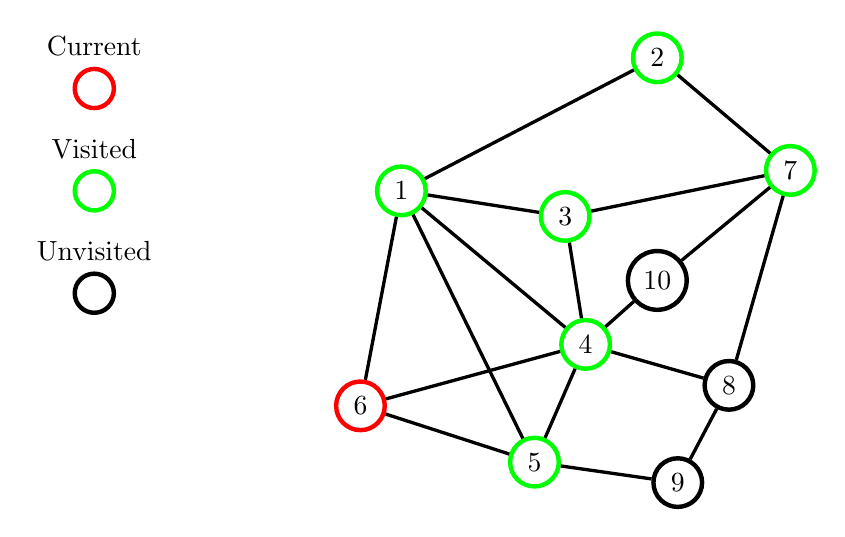
\begin{tikzpicture}[scale=1.3] 
\node[shape=circle, draw=red, 	ultra thick, scale=1.5pt, label={Current}] (U) at (-3, 1) {}; 
\node[shape=circle, draw=green,  ultra thick, scale=1.5pt, label={Visited}] (U) at (-3, 0) {}; 
\node[shape=circle, draw=black, ultra thick, scale=1.5pt, label={Unvisited}] (U) at (-3, -1) {}; 
\node[shape=circle,draw=green, ultra thick] (1) at (0,0) {1}; 
\node[shape=circle,draw=green, ultra thick] (2) at (2.5,1.3) {2}; 
\node[shape=circle,draw=green, ultra thick] (3) at (1.6,-0.25) {3}; 
\node[shape=circle,draw=green, ultra thick] (4) at (1.8,-1.5) {4}; 
\node[shape=circle,draw=green, ultra thick] (5) at (1.3,-2.65) {5}; 
\node[shape=circle,draw=red, ultra thick] (6) at (-0.4,-2.1) {6}; 
\node[shape=circle,draw=green, ultra thick] (7) at (3.8,0.2) {7}; 
\node[shape=circle,draw=black, ultra thick] (8) at (3.2,-1.9) {8}; 
\node[shape=circle,draw=black, ultra thick] (9) at (2.7,-2.85) {9}; 
\node[shape=circle,draw=black, ultra thick] (10) at (2.5,-0.875) {10}; 
\path [-,very thick, draw=black] (2) edge  (1);
\path [-,very thick, draw=black] (3) edge  (1);
\path [-,very thick, draw=black] (4) edge  (1);
\path [-,very thick, draw=black] (5) edge  (1);
\path [-,very thick, draw=black] (6) edge  (1);
\path [-,very thick, draw=black] (7) edge  (2);
\path [-,very thick, draw=black] (7) edge  (3);
\path [-,very thick, draw=black] (4) edge  (3);
\path [-,very thick, draw=black] (5) edge  (4);
\path [-,very thick, draw=black] (6) edge  (4);
\path [-,very thick, draw=black] (8) edge  (4);
\path [-,very thick, draw=black] (10) edge  (4);
\path [-,very thick, draw=black] (6) edge  (5);
\path [-,very thick, draw=black] (9) edge  (5);
\path [-,very thick, draw=black] (8) edge  (7);
\path [-,very thick, draw=black] (10) edge  (7);
\path [-,very thick, draw=black] (9) edge  (8);
\end{tikzpicture} 
\end{figure} 
\end{frame} 
\begin{frame}{DFS : Example}
\begin{figure}
\center
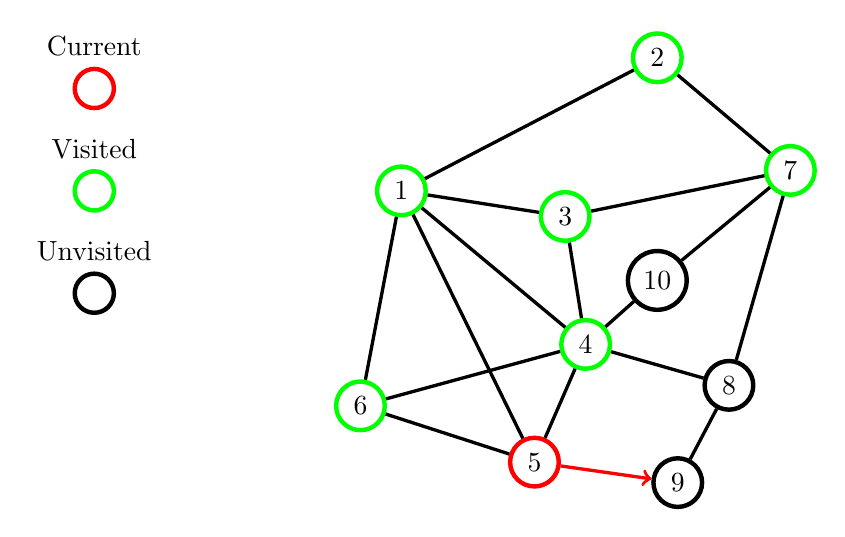
\begin{tikzpicture}[scale=1.3] 
\node[shape=circle, draw=red, 	ultra thick, scale=1.5pt, label={Current}] (U) at (-3, 1) {}; 
\node[shape=circle, draw=green,  ultra thick, scale=1.5pt, label={Visited}] (U) at (-3, 0) {}; 
\node[shape=circle, draw=black, ultra thick, scale=1.5pt, label={Unvisited}] (U) at (-3, -1) {}; 
\node[shape=circle,draw=green, ultra thick] (1) at (0,0) {1}; 
\node[shape=circle,draw=green, ultra thick] (2) at (2.5,1.3) {2}; 
\node[shape=circle,draw=green, ultra thick] (3) at (1.6,-0.25) {3}; 
\node[shape=circle,draw=green, ultra thick] (4) at (1.8,-1.5) {4}; 
\node[shape=circle,draw=red, ultra thick] (5) at (1.3,-2.65) {5}; 
\node[shape=circle,draw=green, ultra thick] (6) at (-0.4,-2.1) {6}; 
\node[shape=circle,draw=green, ultra thick] (7) at (3.8,0.2) {7}; 
\node[shape=circle,draw=black, ultra thick] (8) at (3.2,-1.9) {8}; 
\node[shape=circle,draw=black, ultra thick] (9) at (2.7,-2.85) {9}; 
\node[shape=circle,draw=black, ultra thick] (10) at (2.5,-0.875) {10}; 
\path [-,very thick, draw=black] (2) edge  (1);
\path [-,very thick, draw=black] (3) edge  (1);
\path [-,very thick, draw=black] (4) edge  (1);
\path [-,very thick, draw=black] (5) edge  (1);
\path [-,very thick, draw=black] (6) edge  (1);
\path [-,very thick, draw=black] (7) edge  (2);
\path [-,very thick, draw=black] (7) edge  (3);
\path [-,very thick, draw=black] (4) edge  (3);
\path [-,very thick, draw=black] (5) edge  (4);
\path [-,very thick, draw=black] (6) edge  (4);
\path [-,very thick, draw=black] (8) edge  (4);
\path [-,very thick, draw=black] (10) edge  (4);
\path [-,very thick, draw=black] (6) edge  (5);
\path [-,very thick, draw=black] (8) edge  (7);
\path [-,very thick, draw=black] (10) edge  (7);
\path [-,very thick, draw=black] (9) edge  (8);
\path [->,very thick, draw=red] (5) edge  (9);
\end{tikzpicture} 
\end{figure} 
\end{frame} 
\begin{frame}{DFS : Example}
\begin{figure}
\center
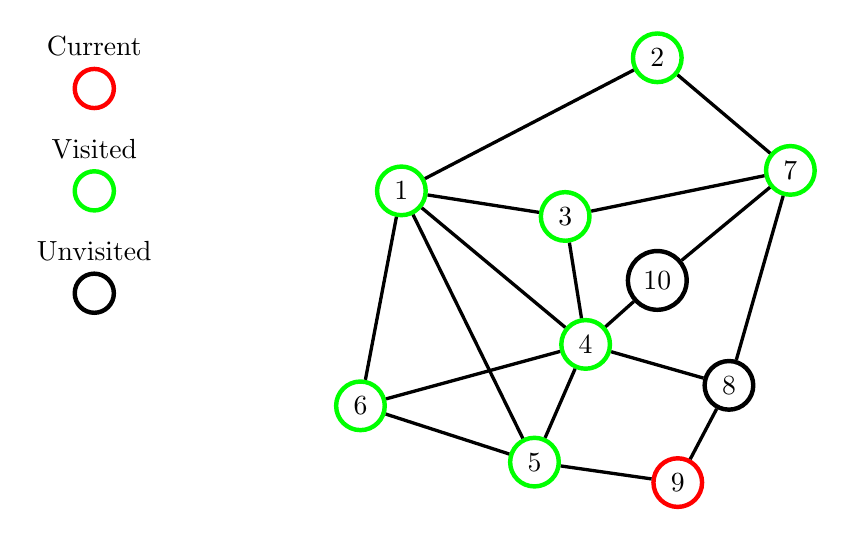
\begin{tikzpicture}[scale=1.3] 
\node[shape=circle, draw=red, 	ultra thick, scale=1.5pt, label={Current}] (U) at (-3, 1) {}; 
\node[shape=circle, draw=green,  ultra thick, scale=1.5pt, label={Visited}] (U) at (-3, 0) {}; 
\node[shape=circle, draw=black, ultra thick, scale=1.5pt, label={Unvisited}] (U) at (-3, -1) {}; 
\node[shape=circle,draw=green, ultra thick] (1) at (0,0) {1}; 
\node[shape=circle,draw=green, ultra thick] (2) at (2.5,1.3) {2}; 
\node[shape=circle,draw=green, ultra thick] (3) at (1.6,-0.25) {3}; 
\node[shape=circle,draw=green, ultra thick] (4) at (1.8,-1.5) {4}; 
\node[shape=circle,draw=green, ultra thick] (5) at (1.3,-2.65) {5}; 
\node[shape=circle,draw=green, ultra thick] (6) at (-0.4,-2.1) {6}; 
\node[shape=circle,draw=green, ultra thick] (7) at (3.8,0.2) {7}; 
\node[shape=circle,draw=black, ultra thick] (8) at (3.2,-1.9) {8}; 
\node[shape=circle,draw=red, ultra thick] (9) at (2.7,-2.85) {9}; 
\node[shape=circle,draw=black, ultra thick] (10) at (2.5,-0.875) {10}; 
\path [-,very thick, draw=black] (2) edge  (1);
\path [-,very thick, draw=black] (3) edge  (1);
\path [-,very thick, draw=black] (4) edge  (1);
\path [-,very thick, draw=black] (5) edge  (1);
\path [-,very thick, draw=black] (6) edge  (1);
\path [-,very thick, draw=black] (7) edge  (2);
\path [-,very thick, draw=black] (7) edge  (3);
\path [-,very thick, draw=black] (4) edge  (3);
\path [-,very thick, draw=black] (5) edge  (4);
\path [-,very thick, draw=black] (6) edge  (4);
\path [-,very thick, draw=black] (8) edge  (4);
\path [-,very thick, draw=black] (10) edge  (4);
\path [-,very thick, draw=black] (6) edge  (5);
\path [-,very thick, draw=black] (9) edge  (5);
\path [-,very thick, draw=black] (8) edge  (7);
\path [-,very thick, draw=black] (10) edge  (7);
\path [-,very thick, draw=black] (9) edge  (8);
\end{tikzpicture} 
\end{figure} 
\end{frame} 
\begin{frame}{DFS : Example}
\begin{figure}
\center
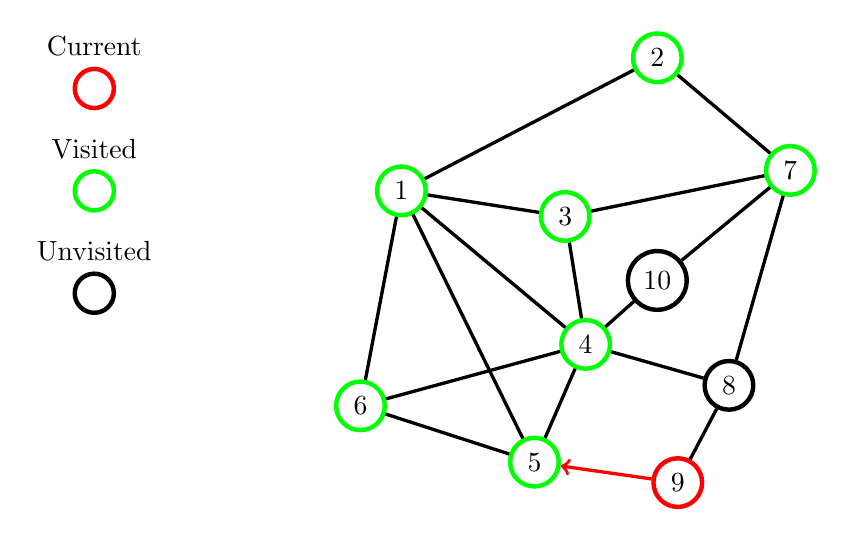
\begin{tikzpicture}[scale=1.3] 
\node[shape=circle, draw=red, 	ultra thick, scale=1.5pt, label={Current}] (U) at (-3, 1) {}; 
\node[shape=circle, draw=green,  ultra thick, scale=1.5pt, label={Visited}] (U) at (-3, 0) {}; 
\node[shape=circle, draw=black, ultra thick, scale=1.5pt, label={Unvisited}] (U) at (-3, -1) {}; 
\node[shape=circle,draw=green, ultra thick] (1) at (0,0) {1}; 
\node[shape=circle,draw=green, ultra thick] (2) at (2.5,1.3) {2}; 
\node[shape=circle,draw=green, ultra thick] (3) at (1.6,-0.25) {3}; 
\node[shape=circle,draw=green, ultra thick] (4) at (1.8,-1.5) {4}; 
\node[shape=circle,draw=green, ultra thick] (5) at (1.3,-2.65) {5}; 
\node[shape=circle,draw=green, ultra thick] (6) at (-0.4,-2.1) {6}; 
\node[shape=circle,draw=green, ultra thick] (7) at (3.8,0.2) {7}; 
\node[shape=circle,draw=black, ultra thick] (8) at (3.2,-1.9) {8}; 
\node[shape=circle,draw=red, ultra thick] (9) at (2.7,-2.85) {9}; 
\node[shape=circle,draw=black, ultra thick] (10) at (2.5,-0.875) {10}; 
\path [-,very thick, draw=black] (2) edge  (1);
\path [-,very thick, draw=black] (3) edge  (1);
\path [-,very thick, draw=black] (4) edge  (1);
\path [-,very thick, draw=black] (5) edge  (1);
\path [-,very thick, draw=black] (6) edge  (1);
\path [-,very thick, draw=black] (7) edge  (2);
\path [-,very thick, draw=black] (7) edge  (3);
\path [-,very thick, draw=black] (4) edge  (3);
\path [-,very thick, draw=black] (5) edge  (4);
\path [-,very thick, draw=black] (6) edge  (4);
\path [-,very thick, draw=black] (8) edge  (4);
\path [-,very thick, draw=black] (10) edge  (4);
\path [-,very thick, draw=black] (6) edge  (5);
\path [-,very thick, draw=black] (8) edge  (7);
\path [-,very thick, draw=black] (10) edge  (7);
\path [-,very thick, draw=black] (9) edge  (8);
\path [->,very thick, draw=red] (9) edge  (5);
\end{tikzpicture} 
\end{figure} 
\end{frame} 
\begin{frame}{DFS : Example}
\begin{figure}
\center
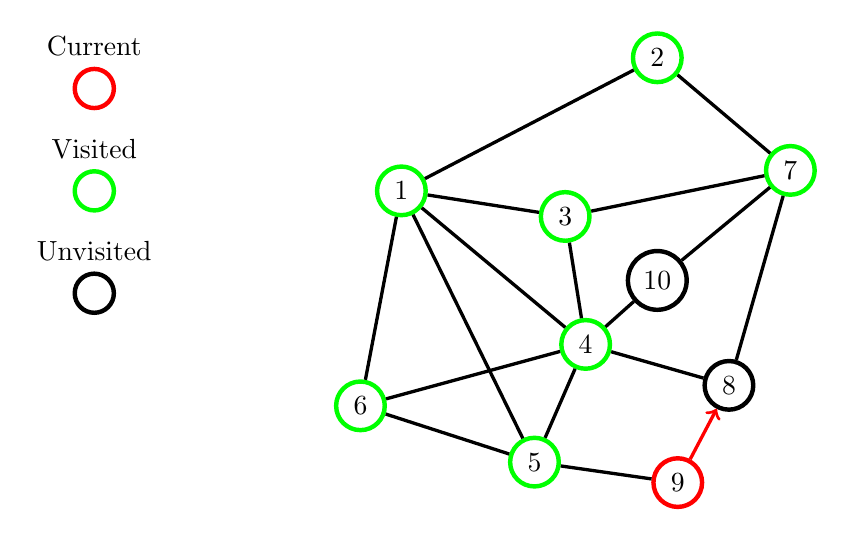
\begin{tikzpicture}[scale=1.3] 
\node[shape=circle, draw=red, 	ultra thick, scale=1.5pt, label={Current}] (U) at (-3, 1) {}; 
\node[shape=circle, draw=green,  ultra thick, scale=1.5pt, label={Visited}] (U) at (-3, 0) {}; 
\node[shape=circle, draw=black, ultra thick, scale=1.5pt, label={Unvisited}] (U) at (-3, -1) {}; 
\node[shape=circle,draw=green, ultra thick] (1) at (0,0) {1}; 
\node[shape=circle,draw=green, ultra thick] (2) at (2.5,1.3) {2}; 
\node[shape=circle,draw=green, ultra thick] (3) at (1.6,-0.25) {3}; 
\node[shape=circle,draw=green, ultra thick] (4) at (1.8,-1.5) {4}; 
\node[shape=circle,draw=green, ultra thick] (5) at (1.3,-2.65) {5}; 
\node[shape=circle,draw=green, ultra thick] (6) at (-0.4,-2.1) {6}; 
\node[shape=circle,draw=green, ultra thick] (7) at (3.8,0.2) {7}; 
\node[shape=circle,draw=black, ultra thick] (8) at (3.2,-1.9) {8}; 
\node[shape=circle,draw=red, ultra thick] (9) at (2.7,-2.85) {9}; 
\node[shape=circle,draw=black, ultra thick] (10) at (2.5,-0.875) {10}; 
\path [-,very thick, draw=black] (2) edge  (1);
\path [-,very thick, draw=black] (3) edge  (1);
\path [-,very thick, draw=black] (4) edge  (1);
\path [-,very thick, draw=black] (5) edge  (1);
\path [-,very thick, draw=black] (6) edge  (1);
\path [-,very thick, draw=black] (7) edge  (2);
\path [-,very thick, draw=black] (7) edge  (3);
\path [-,very thick, draw=black] (4) edge  (3);
\path [-,very thick, draw=black] (5) edge  (4);
\path [-,very thick, draw=black] (6) edge  (4);
\path [-,very thick, draw=black] (8) edge  (4);
\path [-,very thick, draw=black] (10) edge  (4);
\path [-,very thick, draw=black] (6) edge  (5);
\path [-,very thick, draw=black] (9) edge  (5);
\path [-,very thick, draw=black] (8) edge  (7);
\path [-,very thick, draw=black] (10) edge  (7);
\path [->,very thick, draw=red] (9) edge  (8);
\end{tikzpicture} 
\end{figure} 
\end{frame} 
\begin{frame}{DFS : Example}
\begin{figure}
\center
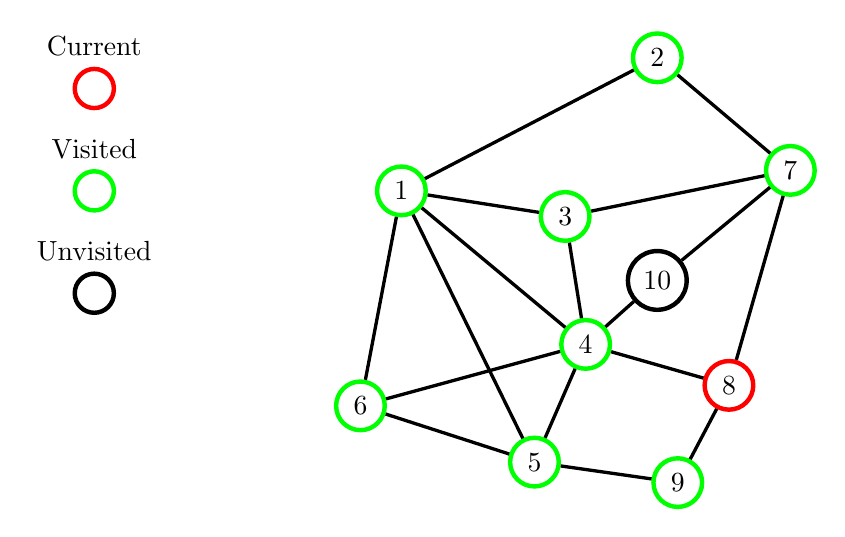
\begin{tikzpicture}[scale=1.3] 
\node[shape=circle, draw=red, 	ultra thick, scale=1.5pt, label={Current}] (U) at (-3, 1) {}; 
\node[shape=circle, draw=green,  ultra thick, scale=1.5pt, label={Visited}] (U) at (-3, 0) {}; 
\node[shape=circle, draw=black, ultra thick, scale=1.5pt, label={Unvisited}] (U) at (-3, -1) {}; 
\node[shape=circle,draw=green, ultra thick] (1) at (0,0) {1}; 
\node[shape=circle,draw=green, ultra thick] (2) at (2.5,1.3) {2}; 
\node[shape=circle,draw=green, ultra thick] (3) at (1.6,-0.25) {3}; 
\node[shape=circle,draw=green, ultra thick] (4) at (1.8,-1.5) {4}; 
\node[shape=circle,draw=green, ultra thick] (5) at (1.3,-2.65) {5}; 
\node[shape=circle,draw=green, ultra thick] (6) at (-0.4,-2.1) {6}; 
\node[shape=circle,draw=green, ultra thick] (7) at (3.8,0.2) {7}; 
\node[shape=circle,draw=red, ultra thick] (8) at (3.2,-1.9) {8}; 
\node[shape=circle,draw=green, ultra thick] (9) at (2.7,-2.85) {9}; 
\node[shape=circle,draw=black, ultra thick] (10) at (2.5,-0.875) {10}; 
\path [-,very thick, draw=black] (2) edge  (1);
\path [-,very thick, draw=black] (3) edge  (1);
\path [-,very thick, draw=black] (4) edge  (1);
\path [-,very thick, draw=black] (5) edge  (1);
\path [-,very thick, draw=black] (6) edge  (1);
\path [-,very thick, draw=black] (7) edge  (2);
\path [-,very thick, draw=black] (7) edge  (3);
\path [-,very thick, draw=black] (4) edge  (3);
\path [-,very thick, draw=black] (5) edge  (4);
\path [-,very thick, draw=black] (6) edge  (4);
\path [-,very thick, draw=black] (8) edge  (4);
\path [-,very thick, draw=black] (10) edge  (4);
\path [-,very thick, draw=black] (6) edge  (5);
\path [-,very thick, draw=black] (9) edge  (5);
\path [-,very thick, draw=black] (8) edge  (7);
\path [-,very thick, draw=black] (10) edge  (7);
\path [-,very thick, draw=black] (9) edge  (8);
\end{tikzpicture} 
\end{figure} 
\end{frame} 
\begin{frame}{DFS : Example}
\begin{figure}
\center
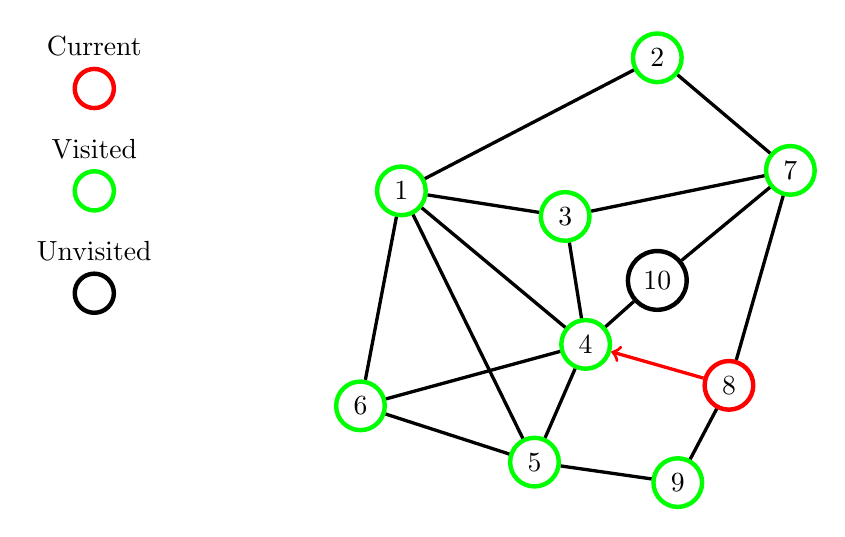
\begin{tikzpicture}[scale=1.3] 
\node[shape=circle, draw=red, 	ultra thick, scale=1.5pt, label={Current}] (U) at (-3, 1) {}; 
\node[shape=circle, draw=green,  ultra thick, scale=1.5pt, label={Visited}] (U) at (-3, 0) {}; 
\node[shape=circle, draw=black, ultra thick, scale=1.5pt, label={Unvisited}] (U) at (-3, -1) {}; 
\node[shape=circle,draw=green, ultra thick] (1) at (0,0) {1}; 
\node[shape=circle,draw=green, ultra thick] (2) at (2.5,1.3) {2}; 
\node[shape=circle,draw=green, ultra thick] (3) at (1.6,-0.25) {3}; 
\node[shape=circle,draw=green, ultra thick] (4) at (1.8,-1.5) {4}; 
\node[shape=circle,draw=green, ultra thick] (5) at (1.3,-2.65) {5}; 
\node[shape=circle,draw=green, ultra thick] (6) at (-0.4,-2.1) {6}; 
\node[shape=circle,draw=green, ultra thick] (7) at (3.8,0.2) {7}; 
\node[shape=circle,draw=red, ultra thick] (8) at (3.2,-1.9) {8}; 
\node[shape=circle,draw=green, ultra thick] (9) at (2.7,-2.85) {9}; 
\node[shape=circle,draw=black, ultra thick] (10) at (2.5,-0.875) {10}; 
\path [-,very thick, draw=black] (2) edge  (1);
\path [-,very thick, draw=black] (3) edge  (1);
\path [-,very thick, draw=black] (4) edge  (1);
\path [-,very thick, draw=black] (5) edge  (1);
\path [-,very thick, draw=black] (6) edge  (1);
\path [-,very thick, draw=black] (7) edge  (2);
\path [-,very thick, draw=black] (7) edge  (3);
\path [-,very thick, draw=black] (4) edge  (3);
\path [-,very thick, draw=black] (5) edge  (4);
\path [-,very thick, draw=black] (6) edge  (4);
\path [-,very thick, draw=black] (10) edge  (4);
\path [-,very thick, draw=black] (6) edge  (5);
\path [-,very thick, draw=black] (9) edge  (5);
\path [-,very thick, draw=black] (8) edge  (7);
\path [-,very thick, draw=black] (10) edge  (7);
\path [-,very thick, draw=black] (9) edge  (8);
\path [->,very thick, draw=red] (8) edge  (4);
\end{tikzpicture} 
\end{figure} 
\end{frame} 
\begin{frame}{DFS : Example}
\begin{figure}
\center
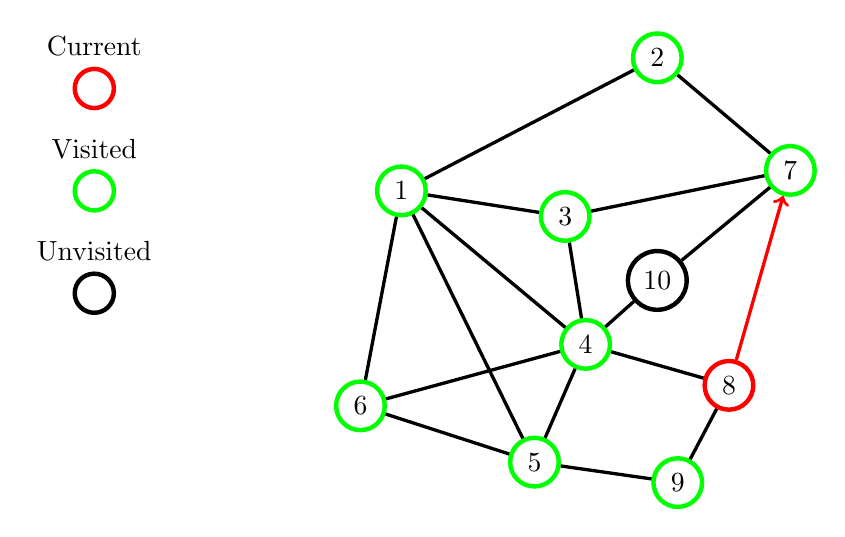
\begin{tikzpicture}[scale=1.3] 
\node[shape=circle, draw=red, 	ultra thick, scale=1.5pt, label={Current}] (U) at (-3, 1) {}; 
\node[shape=circle, draw=green,  ultra thick, scale=1.5pt, label={Visited}] (U) at (-3, 0) {}; 
\node[shape=circle, draw=black, ultra thick, scale=1.5pt, label={Unvisited}] (U) at (-3, -1) {}; 
\node[shape=circle,draw=green, ultra thick] (1) at (0,0) {1}; 
\node[shape=circle,draw=green, ultra thick] (2) at (2.5,1.3) {2}; 
\node[shape=circle,draw=green, ultra thick] (3) at (1.6,-0.25) {3}; 
\node[shape=circle,draw=green, ultra thick] (4) at (1.8,-1.5) {4}; 
\node[shape=circle,draw=green, ultra thick] (5) at (1.3,-2.65) {5}; 
\node[shape=circle,draw=green, ultra thick] (6) at (-0.4,-2.1) {6}; 
\node[shape=circle,draw=green, ultra thick] (7) at (3.8,0.2) {7}; 
\node[shape=circle,draw=red, ultra thick] (8) at (3.2,-1.9) {8}; 
\node[shape=circle,draw=green, ultra thick] (9) at (2.7,-2.85) {9}; 
\node[shape=circle,draw=black, ultra thick] (10) at (2.5,-0.875) {10}; 
\path [-,very thick, draw=black] (2) edge  (1);
\path [-,very thick, draw=black] (3) edge  (1);
\path [-,very thick, draw=black] (4) edge  (1);
\path [-,very thick, draw=black] (5) edge  (1);
\path [-,very thick, draw=black] (6) edge  (1);
\path [-,very thick, draw=black] (7) edge  (2);
\path [-,very thick, draw=black] (7) edge  (3);
\path [-,very thick, draw=black] (4) edge  (3);
\path [-,very thick, draw=black] (5) edge  (4);
\path [-,very thick, draw=black] (6) edge  (4);
\path [-,very thick, draw=black] (8) edge  (4);
\path [-,very thick, draw=black] (10) edge  (4);
\path [-,very thick, draw=black] (6) edge  (5);
\path [-,very thick, draw=black] (9) edge  (5);
\path [-,very thick, draw=black] (10) edge  (7);
\path [-,very thick, draw=black] (9) edge  (8);
\path [->,very thick, draw=red] (8) edge  (7);
\end{tikzpicture} 
\end{figure} 
\end{frame} 
\begin{frame}{DFS : Example}
\begin{figure}
\center
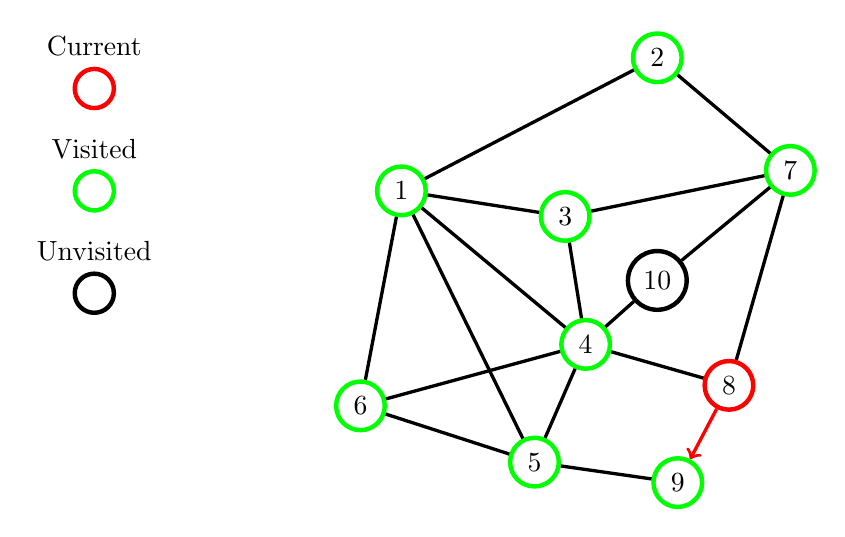
\begin{tikzpicture}[scale=1.3] 
\node[shape=circle, draw=red, 	ultra thick, scale=1.5pt, label={Current}] (U) at (-3, 1) {}; 
\node[shape=circle, draw=green,  ultra thick, scale=1.5pt, label={Visited}] (U) at (-3, 0) {}; 
\node[shape=circle, draw=black, ultra thick, scale=1.5pt, label={Unvisited}] (U) at (-3, -1) {}; 
\node[shape=circle,draw=green, ultra thick] (1) at (0,0) {1}; 
\node[shape=circle,draw=green, ultra thick] (2) at (2.5,1.3) {2}; 
\node[shape=circle,draw=green, ultra thick] (3) at (1.6,-0.25) {3}; 
\node[shape=circle,draw=green, ultra thick] (4) at (1.8,-1.5) {4}; 
\node[shape=circle,draw=green, ultra thick] (5) at (1.3,-2.65) {5}; 
\node[shape=circle,draw=green, ultra thick] (6) at (-0.4,-2.1) {6}; 
\node[shape=circle,draw=green, ultra thick] (7) at (3.8,0.2) {7}; 
\node[shape=circle,draw=red, ultra thick] (8) at (3.2,-1.9) {8}; 
\node[shape=circle,draw=green, ultra thick] (9) at (2.7,-2.85) {9}; 
\node[shape=circle,draw=black, ultra thick] (10) at (2.5,-0.875) {10}; 
\path [-,very thick, draw=black] (2) edge  (1);
\path [-,very thick, draw=black] (3) edge  (1);
\path [-,very thick, draw=black] (4) edge  (1);
\path [-,very thick, draw=black] (5) edge  (1);
\path [-,very thick, draw=black] (6) edge  (1);
\path [-,very thick, draw=black] (7) edge  (2);
\path [-,very thick, draw=black] (7) edge  (3);
\path [-,very thick, draw=black] (4) edge  (3);
\path [-,very thick, draw=black] (5) edge  (4);
\path [-,very thick, draw=black] (6) edge  (4);
\path [-,very thick, draw=black] (8) edge  (4);
\path [-,very thick, draw=black] (10) edge  (4);
\path [-,very thick, draw=black] (6) edge  (5);
\path [-,very thick, draw=black] (9) edge  (5);
\path [-,very thick, draw=black] (8) edge  (7);
\path [-,very thick, draw=black] (10) edge  (7);
\path [->,very thick, draw=red] (8) edge  (9);
\end{tikzpicture} 
\end{figure} 
\end{frame} 
\begin{frame}{DFS : Example}
\begin{figure}
\center
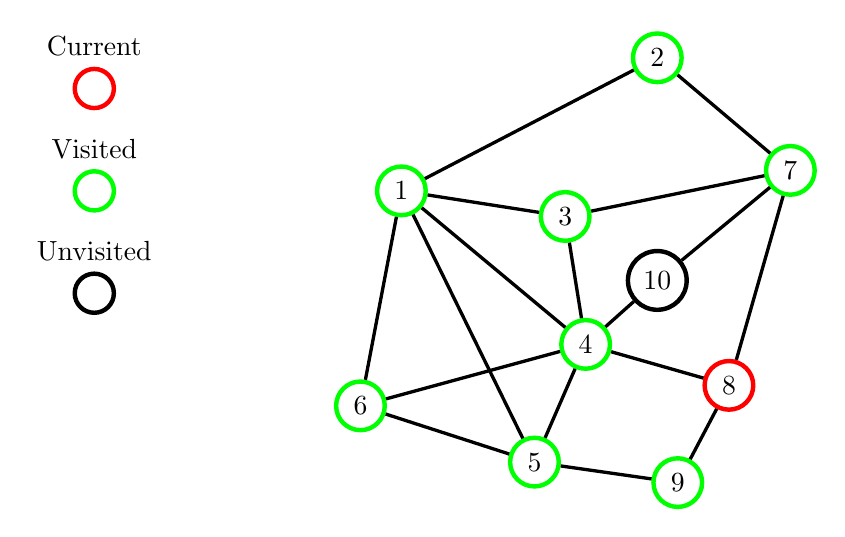
\begin{tikzpicture}[scale=1.3] 
\node[shape=circle, draw=red, 	ultra thick, scale=1.5pt, label={Current}] (U) at (-3, 1) {}; 
\node[shape=circle, draw=green,  ultra thick, scale=1.5pt, label={Visited}] (U) at (-3, 0) {}; 
\node[shape=circle, draw=black, ultra thick, scale=1.5pt, label={Unvisited}] (U) at (-3, -1) {}; 
\node[shape=circle,draw=green, ultra thick] (1) at (0,0) {1}; 
\node[shape=circle,draw=green, ultra thick] (2) at (2.5,1.3) {2}; 
\node[shape=circle,draw=green, ultra thick] (3) at (1.6,-0.25) {3}; 
\node[shape=circle,draw=green, ultra thick] (4) at (1.8,-1.5) {4}; 
\node[shape=circle,draw=green, ultra thick] (5) at (1.3,-2.65) {5}; 
\node[shape=circle,draw=green, ultra thick] (6) at (-0.4,-2.1) {6}; 
\node[shape=circle,draw=green, ultra thick] (7) at (3.8,0.2) {7}; 
\node[shape=circle,draw=red, ultra thick] (8) at (3.2,-1.9) {8}; 
\node[shape=circle,draw=green, ultra thick] (9) at (2.7,-2.85) {9}; 
\node[shape=circle,draw=black, ultra thick] (10) at (2.5,-0.875) {10}; 
\path [-,very thick, draw=black] (2) edge  (1);
\path [-,very thick, draw=black] (3) edge  (1);
\path [-,very thick, draw=black] (4) edge  (1);
\path [-,very thick, draw=black] (5) edge  (1);
\path [-,very thick, draw=black] (6) edge  (1);
\path [-,very thick, draw=black] (7) edge  (2);
\path [-,very thick, draw=black] (7) edge  (3);
\path [-,very thick, draw=black] (4) edge  (3);
\path [-,very thick, draw=black] (5) edge  (4);
\path [-,very thick, draw=black] (6) edge  (4);
\path [-,very thick, draw=black] (8) edge  (4);
\path [-,very thick, draw=black] (10) edge  (4);
\path [-,very thick, draw=black] (6) edge  (5);
\path [-,very thick, draw=black] (9) edge  (5);
\path [-,very thick, draw=black] (8) edge  (7);
\path [-,very thick, draw=black] (10) edge  (7);
\path [-,very thick, draw=black] (9) edge  (8);
\end{tikzpicture} 
\end{figure} 
\end{frame} 
\begin{frame}{DFS : Example}
\begin{figure}
\center
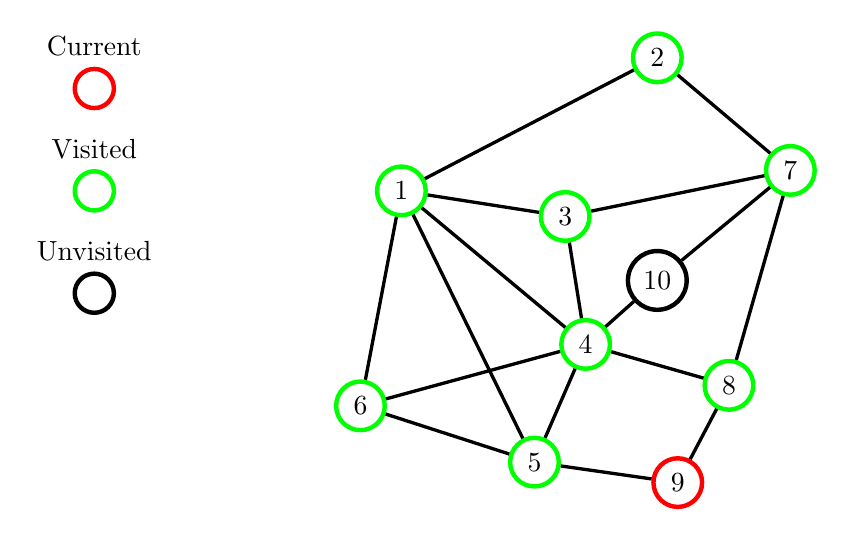
\begin{tikzpicture}[scale=1.3] 
\node[shape=circle, draw=red, 	ultra thick, scale=1.5pt, label={Current}] (U) at (-3, 1) {}; 
\node[shape=circle, draw=green,  ultra thick, scale=1.5pt, label={Visited}] (U) at (-3, 0) {}; 
\node[shape=circle, draw=black, ultra thick, scale=1.5pt, label={Unvisited}] (U) at (-3, -1) {}; 
\node[shape=circle,draw=green, ultra thick] (1) at (0,0) {1}; 
\node[shape=circle,draw=green, ultra thick] (2) at (2.5,1.3) {2}; 
\node[shape=circle,draw=green, ultra thick] (3) at (1.6,-0.25) {3}; 
\node[shape=circle,draw=green, ultra thick] (4) at (1.8,-1.5) {4}; 
\node[shape=circle,draw=green, ultra thick] (5) at (1.3,-2.65) {5}; 
\node[shape=circle,draw=green, ultra thick] (6) at (-0.4,-2.1) {6}; 
\node[shape=circle,draw=green, ultra thick] (7) at (3.8,0.2) {7}; 
\node[shape=circle,draw=green, ultra thick] (8) at (3.2,-1.9) {8}; 
\node[shape=circle,draw=red, ultra thick] (9) at (2.7,-2.85) {9}; 
\node[shape=circle,draw=black, ultra thick] (10) at (2.5,-0.875) {10}; 
\path [-,very thick, draw=black] (2) edge  (1);
\path [-,very thick, draw=black] (3) edge  (1);
\path [-,very thick, draw=black] (4) edge  (1);
\path [-,very thick, draw=black] (5) edge  (1);
\path [-,very thick, draw=black] (6) edge  (1);
\path [-,very thick, draw=black] (7) edge  (2);
\path [-,very thick, draw=black] (7) edge  (3);
\path [-,very thick, draw=black] (4) edge  (3);
\path [-,very thick, draw=black] (5) edge  (4);
\path [-,very thick, draw=black] (6) edge  (4);
\path [-,very thick, draw=black] (8) edge  (4);
\path [-,very thick, draw=black] (10) edge  (4);
\path [-,very thick, draw=black] (6) edge  (5);
\path [-,very thick, draw=black] (9) edge  (5);
\path [-,very thick, draw=black] (8) edge  (7);
\path [-,very thick, draw=black] (10) edge  (7);
\path [-,very thick, draw=black] (9) edge  (8);
\end{tikzpicture} 
\end{figure} 
\end{frame} 
\begin{frame}{DFS : Example}
\begin{figure}
\center
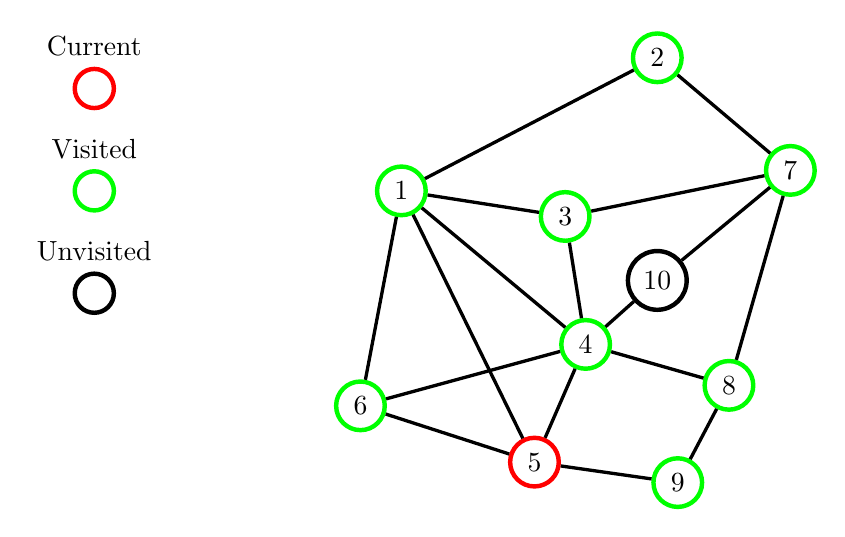
\begin{tikzpicture}[scale=1.3] 
\node[shape=circle, draw=red, 	ultra thick, scale=1.5pt, label={Current}] (U) at (-3, 1) {}; 
\node[shape=circle, draw=green,  ultra thick, scale=1.5pt, label={Visited}] (U) at (-3, 0) {}; 
\node[shape=circle, draw=black, ultra thick, scale=1.5pt, label={Unvisited}] (U) at (-3, -1) {}; 
\node[shape=circle,draw=green, ultra thick] (1) at (0,0) {1}; 
\node[shape=circle,draw=green, ultra thick] (2) at (2.5,1.3) {2}; 
\node[shape=circle,draw=green, ultra thick] (3) at (1.6,-0.25) {3}; 
\node[shape=circle,draw=green, ultra thick] (4) at (1.8,-1.5) {4}; 
\node[shape=circle,draw=red, ultra thick] (5) at (1.3,-2.65) {5}; 
\node[shape=circle,draw=green, ultra thick] (6) at (-0.4,-2.1) {6}; 
\node[shape=circle,draw=green, ultra thick] (7) at (3.8,0.2) {7}; 
\node[shape=circle,draw=green, ultra thick] (8) at (3.2,-1.9) {8}; 
\node[shape=circle,draw=green, ultra thick] (9) at (2.7,-2.85) {9}; 
\node[shape=circle,draw=black, ultra thick] (10) at (2.5,-0.875) {10}; 
\path [-,very thick, draw=black] (2) edge  (1);
\path [-,very thick, draw=black] (3) edge  (1);
\path [-,very thick, draw=black] (4) edge  (1);
\path [-,very thick, draw=black] (5) edge  (1);
\path [-,very thick, draw=black] (6) edge  (1);
\path [-,very thick, draw=black] (7) edge  (2);
\path [-,very thick, draw=black] (7) edge  (3);
\path [-,very thick, draw=black] (4) edge  (3);
\path [-,very thick, draw=black] (5) edge  (4);
\path [-,very thick, draw=black] (6) edge  (4);
\path [-,very thick, draw=black] (8) edge  (4);
\path [-,very thick, draw=black] (10) edge  (4);
\path [-,very thick, draw=black] (6) edge  (5);
\path [-,very thick, draw=black] (9) edge  (5);
\path [-,very thick, draw=black] (8) edge  (7);
\path [-,very thick, draw=black] (10) edge  (7);
\path [-,very thick, draw=black] (9) edge  (8);
\end{tikzpicture} 
\end{figure} 
\end{frame} 
\begin{frame}{DFS : Example}
\begin{figure}
\center
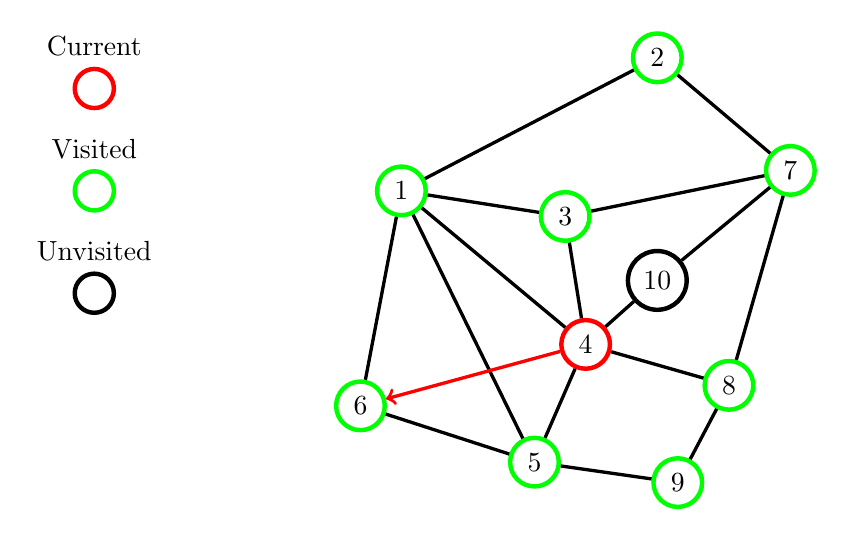
\begin{tikzpicture}[scale=1.3] 
\node[shape=circle, draw=red, 	ultra thick, scale=1.5pt, label={Current}] (U) at (-3, 1) {}; 
\node[shape=circle, draw=green,  ultra thick, scale=1.5pt, label={Visited}] (U) at (-3, 0) {}; 
\node[shape=circle, draw=black, ultra thick, scale=1.5pt, label={Unvisited}] (U) at (-3, -1) {}; 
\node[shape=circle,draw=green, ultra thick] (1) at (0,0) {1}; 
\node[shape=circle,draw=green, ultra thick] (2) at (2.5,1.3) {2}; 
\node[shape=circle,draw=green, ultra thick] (3) at (1.6,-0.25) {3}; 
\node[shape=circle,draw=red, ultra thick] (4) at (1.8,-1.5) {4}; 
\node[shape=circle,draw=green, ultra thick] (5) at (1.3,-2.65) {5}; 
\node[shape=circle,draw=green, ultra thick] (6) at (-0.4,-2.1) {6}; 
\node[shape=circle,draw=green, ultra thick] (7) at (3.8,0.2) {7}; 
\node[shape=circle,draw=green, ultra thick] (8) at (3.2,-1.9) {8}; 
\node[shape=circle,draw=green, ultra thick] (9) at (2.7,-2.85) {9}; 
\node[shape=circle,draw=black, ultra thick] (10) at (2.5,-0.875) {10}; 
\path [-,very thick, draw=black] (2) edge  (1);
\path [-,very thick, draw=black] (3) edge  (1);
\path [-,very thick, draw=black] (4) edge  (1);
\path [-,very thick, draw=black] (5) edge  (1);
\path [-,very thick, draw=black] (6) edge  (1);
\path [-,very thick, draw=black] (7) edge  (2);
\path [-,very thick, draw=black] (7) edge  (3);
\path [-,very thick, draw=black] (4) edge  (3);
\path [-,very thick, draw=black] (5) edge  (4);
\path [-,very thick, draw=black] (8) edge  (4);
\path [-,very thick, draw=black] (10) edge  (4);
\path [-,very thick, draw=black] (6) edge  (5);
\path [-,very thick, draw=black] (9) edge  (5);
\path [-,very thick, draw=black] (8) edge  (7);
\path [-,very thick, draw=black] (10) edge  (7);
\path [-,very thick, draw=black] (9) edge  (8);
\path [->,very thick, draw=red] (4) edge  (6);
\end{tikzpicture} 
\end{figure} 
\end{frame} 
\begin{frame}{DFS : Example}
\begin{figure}
\center
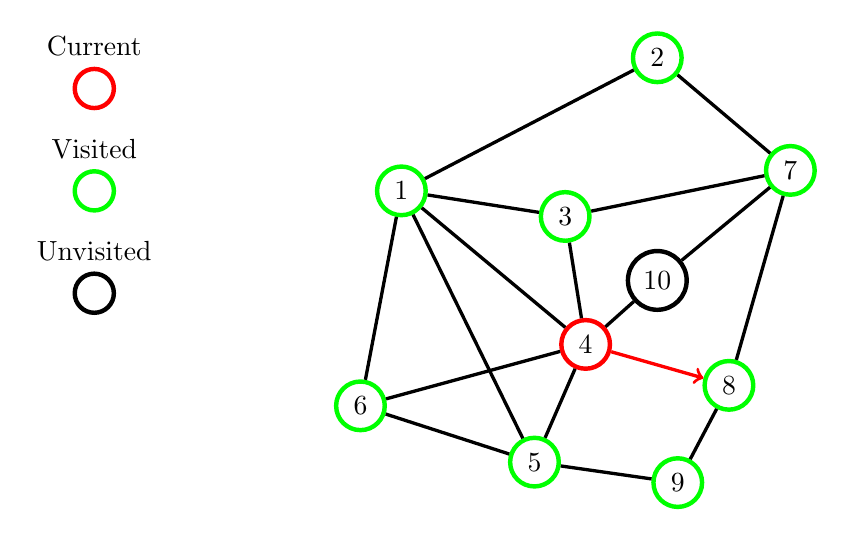
\begin{tikzpicture}[scale=1.3] 
\node[shape=circle, draw=red, 	ultra thick, scale=1.5pt, label={Current}] (U) at (-3, 1) {}; 
\node[shape=circle, draw=green,  ultra thick, scale=1.5pt, label={Visited}] (U) at (-3, 0) {}; 
\node[shape=circle, draw=black, ultra thick, scale=1.5pt, label={Unvisited}] (U) at (-3, -1) {}; 
\node[shape=circle,draw=green, ultra thick] (1) at (0,0) {1}; 
\node[shape=circle,draw=green, ultra thick] (2) at (2.5,1.3) {2}; 
\node[shape=circle,draw=green, ultra thick] (3) at (1.6,-0.25) {3}; 
\node[shape=circle,draw=red, ultra thick] (4) at (1.8,-1.5) {4}; 
\node[shape=circle,draw=green, ultra thick] (5) at (1.3,-2.65) {5}; 
\node[shape=circle,draw=green, ultra thick] (6) at (-0.4,-2.1) {6}; 
\node[shape=circle,draw=green, ultra thick] (7) at (3.8,0.2) {7}; 
\node[shape=circle,draw=green, ultra thick] (8) at (3.2,-1.9) {8}; 
\node[shape=circle,draw=green, ultra thick] (9) at (2.7,-2.85) {9}; 
\node[shape=circle,draw=black, ultra thick] (10) at (2.5,-0.875) {10}; 
\path [-,very thick, draw=black] (2) edge  (1);
\path [-,very thick, draw=black] (3) edge  (1);
\path [-,very thick, draw=black] (4) edge  (1);
\path [-,very thick, draw=black] (5) edge  (1);
\path [-,very thick, draw=black] (6) edge  (1);
\path [-,very thick, draw=black] (7) edge  (2);
\path [-,very thick, draw=black] (7) edge  (3);
\path [-,very thick, draw=black] (4) edge  (3);
\path [-,very thick, draw=black] (5) edge  (4);
\path [-,very thick, draw=black] (6) edge  (4);
\path [-,very thick, draw=black] (10) edge  (4);
\path [-,very thick, draw=black] (6) edge  (5);
\path [-,very thick, draw=black] (9) edge  (5);
\path [-,very thick, draw=black] (8) edge  (7);
\path [-,very thick, draw=black] (10) edge  (7);
\path [-,very thick, draw=black] (9) edge  (8);
\path [->,very thick, draw=red] (4) edge  (8);
\end{tikzpicture} 
\end{figure} 
\end{frame} 
\begin{frame}{DFS : Example}
\begin{figure}
\center
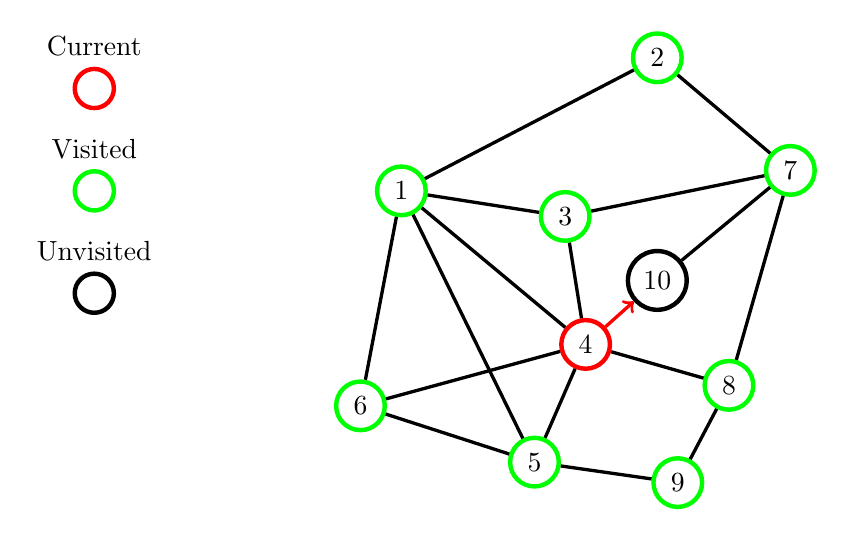
\begin{tikzpicture}[scale=1.3] 
\node[shape=circle, draw=red, 	ultra thick, scale=1.5pt, label={Current}] (U) at (-3, 1) {}; 
\node[shape=circle, draw=green,  ultra thick, scale=1.5pt, label={Visited}] (U) at (-3, 0) {}; 
\node[shape=circle, draw=black, ultra thick, scale=1.5pt, label={Unvisited}] (U) at (-3, -1) {}; 
\node[shape=circle,draw=green, ultra thick] (1) at (0,0) {1}; 
\node[shape=circle,draw=green, ultra thick] (2) at (2.5,1.3) {2}; 
\node[shape=circle,draw=green, ultra thick] (3) at (1.6,-0.25) {3}; 
\node[shape=circle,draw=red, ultra thick] (4) at (1.8,-1.5) {4}; 
\node[shape=circle,draw=green, ultra thick] (5) at (1.3,-2.65) {5}; 
\node[shape=circle,draw=green, ultra thick] (6) at (-0.4,-2.1) {6}; 
\node[shape=circle,draw=green, ultra thick] (7) at (3.8,0.2) {7}; 
\node[shape=circle,draw=green, ultra thick] (8) at (3.2,-1.9) {8}; 
\node[shape=circle,draw=green, ultra thick] (9) at (2.7,-2.85) {9}; 
\node[shape=circle,draw=black, ultra thick] (10) at (2.5,-0.875) {10}; 
\path [-,very thick, draw=black] (2) edge  (1);
\path [-,very thick, draw=black] (3) edge  (1);
\path [-,very thick, draw=black] (4) edge  (1);
\path [-,very thick, draw=black] (5) edge  (1);
\path [-,very thick, draw=black] (6) edge  (1);
\path [-,very thick, draw=black] (7) edge  (2);
\path [-,very thick, draw=black] (7) edge  (3);
\path [-,very thick, draw=black] (4) edge  (3);
\path [-,very thick, draw=black] (5) edge  (4);
\path [-,very thick, draw=black] (6) edge  (4);
\path [-,very thick, draw=black] (8) edge  (4);
\path [-,very thick, draw=black] (6) edge  (5);
\path [-,very thick, draw=black] (9) edge  (5);
\path [-,very thick, draw=black] (8) edge  (7);
\path [-,very thick, draw=black] (10) edge  (7);
\path [-,very thick, draw=black] (9) edge  (8);
\path [->,very thick, draw=red] (4) edge  (10);
\end{tikzpicture} 
\end{figure} 
\end{frame} 
\begin{frame}{DFS : Example}
\begin{figure}
\center
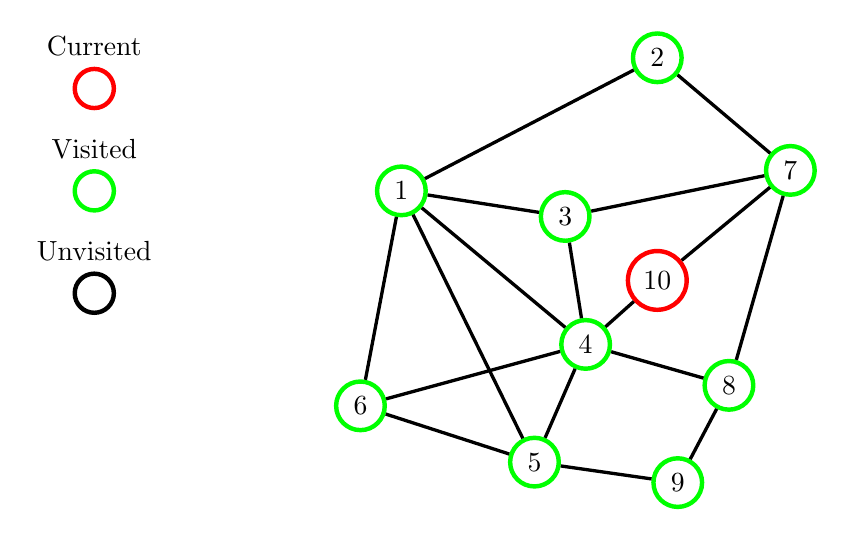
\begin{tikzpicture}[scale=1.3] 
\node[shape=circle, draw=red, 	ultra thick, scale=1.5pt, label={Current}] (U) at (-3, 1) {}; 
\node[shape=circle, draw=green,  ultra thick, scale=1.5pt, label={Visited}] (U) at (-3, 0) {}; 
\node[shape=circle, draw=black, ultra thick, scale=1.5pt, label={Unvisited}] (U) at (-3, -1) {}; 
\node[shape=circle,draw=green, ultra thick] (1) at (0,0) {1}; 
\node[shape=circle,draw=green, ultra thick] (2) at (2.5,1.3) {2}; 
\node[shape=circle,draw=green, ultra thick] (3) at (1.6,-0.25) {3}; 
\node[shape=circle,draw=green, ultra thick] (4) at (1.8,-1.5) {4}; 
\node[shape=circle,draw=green, ultra thick] (5) at (1.3,-2.65) {5}; 
\node[shape=circle,draw=green, ultra thick] (6) at (-0.4,-2.1) {6}; 
\node[shape=circle,draw=green, ultra thick] (7) at (3.8,0.2) {7}; 
\node[shape=circle,draw=green, ultra thick] (8) at (3.2,-1.9) {8}; 
\node[shape=circle,draw=green, ultra thick] (9) at (2.7,-2.85) {9}; 
\node[shape=circle,draw=red, ultra thick] (10) at (2.5,-0.875) {10}; 
\path [-,very thick, draw=black] (2) edge  (1);
\path [-,very thick, draw=black] (3) edge  (1);
\path [-,very thick, draw=black] (4) edge  (1);
\path [-,very thick, draw=black] (5) edge  (1);
\path [-,very thick, draw=black] (6) edge  (1);
\path [-,very thick, draw=black] (7) edge  (2);
\path [-,very thick, draw=black] (7) edge  (3);
\path [-,very thick, draw=black] (4) edge  (3);
\path [-,very thick, draw=black] (5) edge  (4);
\path [-,very thick, draw=black] (6) edge  (4);
\path [-,very thick, draw=black] (8) edge  (4);
\path [-,very thick, draw=black] (10) edge  (4);
\path [-,very thick, draw=black] (6) edge  (5);
\path [-,very thick, draw=black] (9) edge  (5);
\path [-,very thick, draw=black] (8) edge  (7);
\path [-,very thick, draw=black] (10) edge  (7);
\path [-,very thick, draw=black] (9) edge  (8);
\end{tikzpicture} 
\end{figure} 
\end{frame} 
\begin{frame}{DFS : Example}
\begin{figure}
\center
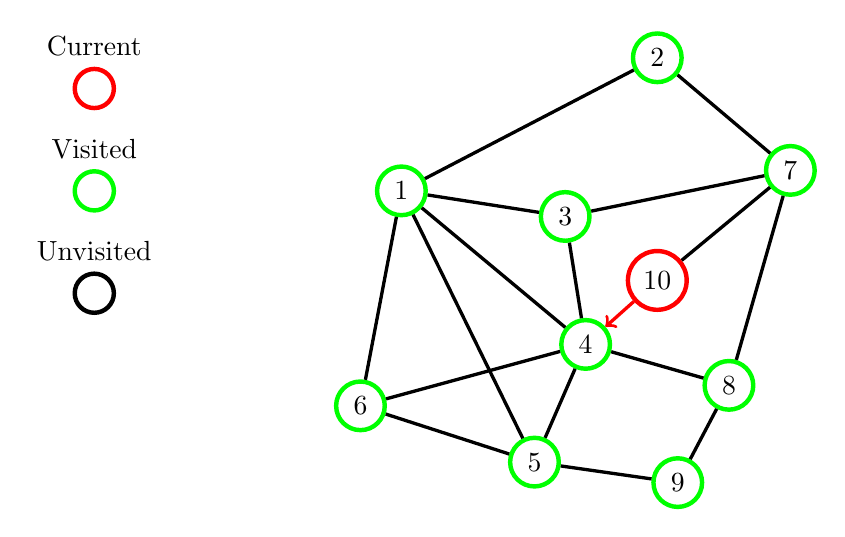
\begin{tikzpicture}[scale=1.3] 
\node[shape=circle, draw=red, 	ultra thick, scale=1.5pt, label={Current}] (U) at (-3, 1) {}; 
\node[shape=circle, draw=green,  ultra thick, scale=1.5pt, label={Visited}] (U) at (-3, 0) {}; 
\node[shape=circle, draw=black, ultra thick, scale=1.5pt, label={Unvisited}] (U) at (-3, -1) {}; 
\node[shape=circle,draw=green, ultra thick] (1) at (0,0) {1}; 
\node[shape=circle,draw=green, ultra thick] (2) at (2.5,1.3) {2}; 
\node[shape=circle,draw=green, ultra thick] (3) at (1.6,-0.25) {3}; 
\node[shape=circle,draw=green, ultra thick] (4) at (1.8,-1.5) {4}; 
\node[shape=circle,draw=green, ultra thick] (5) at (1.3,-2.65) {5}; 
\node[shape=circle,draw=green, ultra thick] (6) at (-0.4,-2.1) {6}; 
\node[shape=circle,draw=green, ultra thick] (7) at (3.8,0.2) {7}; 
\node[shape=circle,draw=green, ultra thick] (8) at (3.2,-1.9) {8}; 
\node[shape=circle,draw=green, ultra thick] (9) at (2.7,-2.85) {9}; 
\node[shape=circle,draw=red, ultra thick] (10) at (2.5,-0.875) {10}; 
\path [-,very thick, draw=black] (2) edge  (1);
\path [-,very thick, draw=black] (3) edge  (1);
\path [-,very thick, draw=black] (4) edge  (1);
\path [-,very thick, draw=black] (5) edge  (1);
\path [-,very thick, draw=black] (6) edge  (1);
\path [-,very thick, draw=black] (7) edge  (2);
\path [-,very thick, draw=black] (7) edge  (3);
\path [-,very thick, draw=black] (4) edge  (3);
\path [-,very thick, draw=black] (5) edge  (4);
\path [-,very thick, draw=black] (6) edge  (4);
\path [-,very thick, draw=black] (8) edge  (4);
\path [-,very thick, draw=black] (6) edge  (5);
\path [-,very thick, draw=black] (9) edge  (5);
\path [-,very thick, draw=black] (8) edge  (7);
\path [-,very thick, draw=black] (10) edge  (7);
\path [-,very thick, draw=black] (9) edge  (8);
\path [->,very thick, draw=red] (10) edge  (4);
\end{tikzpicture} 
\end{figure} 
\end{frame} 
\begin{frame}{DFS : Example}
\begin{figure}
\center
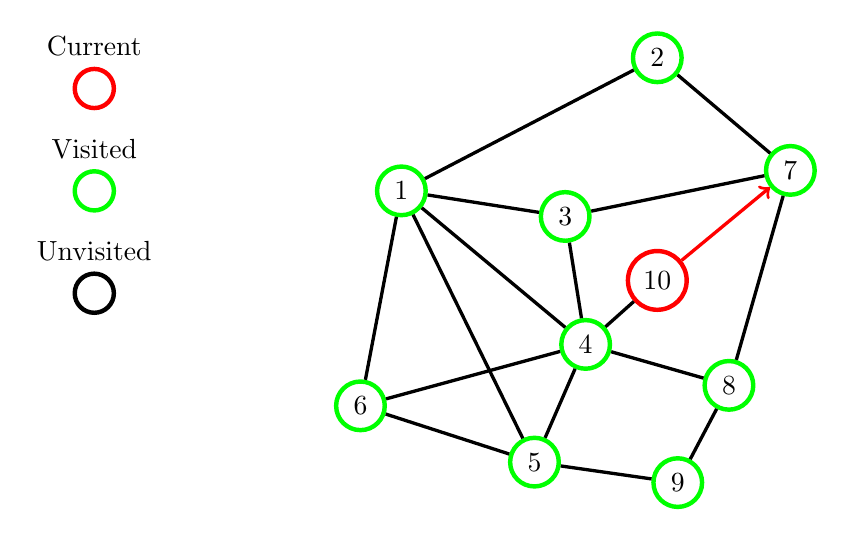
\begin{tikzpicture}[scale=1.3] 
\node[shape=circle, draw=red, 	ultra thick, scale=1.5pt, label={Current}] (U) at (-3, 1) {}; 
\node[shape=circle, draw=green,  ultra thick, scale=1.5pt, label={Visited}] (U) at (-3, 0) {}; 
\node[shape=circle, draw=black, ultra thick, scale=1.5pt, label={Unvisited}] (U) at (-3, -1) {}; 
\node[shape=circle,draw=green, ultra thick] (1) at (0,0) {1}; 
\node[shape=circle,draw=green, ultra thick] (2) at (2.5,1.3) {2}; 
\node[shape=circle,draw=green, ultra thick] (3) at (1.6,-0.25) {3}; 
\node[shape=circle,draw=green, ultra thick] (4) at (1.8,-1.5) {4}; 
\node[shape=circle,draw=green, ultra thick] (5) at (1.3,-2.65) {5}; 
\node[shape=circle,draw=green, ultra thick] (6) at (-0.4,-2.1) {6}; 
\node[shape=circle,draw=green, ultra thick] (7) at (3.8,0.2) {7}; 
\node[shape=circle,draw=green, ultra thick] (8) at (3.2,-1.9) {8}; 
\node[shape=circle,draw=green, ultra thick] (9) at (2.7,-2.85) {9}; 
\node[shape=circle,draw=red, ultra thick] (10) at (2.5,-0.875) {10}; 
\path [-,very thick, draw=black] (2) edge  (1);
\path [-,very thick, draw=black] (3) edge  (1);
\path [-,very thick, draw=black] (4) edge  (1);
\path [-,very thick, draw=black] (5) edge  (1);
\path [-,very thick, draw=black] (6) edge  (1);
\path [-,very thick, draw=black] (7) edge  (2);
\path [-,very thick, draw=black] (7) edge  (3);
\path [-,very thick, draw=black] (4) edge  (3);
\path [-,very thick, draw=black] (5) edge  (4);
\path [-,very thick, draw=black] (6) edge  (4);
\path [-,very thick, draw=black] (8) edge  (4);
\path [-,very thick, draw=black] (10) edge  (4);
\path [-,very thick, draw=black] (6) edge  (5);
\path [-,very thick, draw=black] (9) edge  (5);
\path [-,very thick, draw=black] (8) edge  (7);
\path [-,very thick, draw=black] (9) edge  (8);
\path [->,very thick, draw=red] (10) edge  (7);
\end{tikzpicture} 
\end{figure} 
\end{frame} 
\begin{frame}{DFS : Example}
\begin{figure}
\center
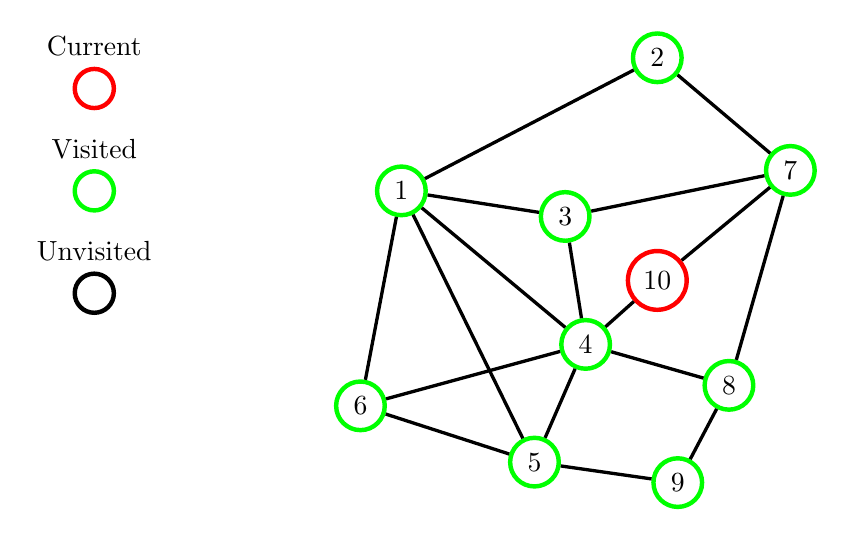
\begin{tikzpicture}[scale=1.3] 
\node[shape=circle, draw=red, 	ultra thick, scale=1.5pt, label={Current}] (U) at (-3, 1) {}; 
\node[shape=circle, draw=green,  ultra thick, scale=1.5pt, label={Visited}] (U) at (-3, 0) {}; 
\node[shape=circle, draw=black, ultra thick, scale=1.5pt, label={Unvisited}] (U) at (-3, -1) {}; 
\node[shape=circle,draw=green, ultra thick] (1) at (0,0) {1}; 
\node[shape=circle,draw=green, ultra thick] (2) at (2.5,1.3) {2}; 
\node[shape=circle,draw=green, ultra thick] (3) at (1.6,-0.25) {3}; 
\node[shape=circle,draw=green, ultra thick] (4) at (1.8,-1.5) {4}; 
\node[shape=circle,draw=green, ultra thick] (5) at (1.3,-2.65) {5}; 
\node[shape=circle,draw=green, ultra thick] (6) at (-0.4,-2.1) {6}; 
\node[shape=circle,draw=green, ultra thick] (7) at (3.8,0.2) {7}; 
\node[shape=circle,draw=green, ultra thick] (8) at (3.2,-1.9) {8}; 
\node[shape=circle,draw=green, ultra thick] (9) at (2.7,-2.85) {9}; 
\node[shape=circle,draw=red, ultra thick] (10) at (2.5,-0.875) {10}; 
\path [-,very thick, draw=black] (2) edge  (1);
\path [-,very thick, draw=black] (3) edge  (1);
\path [-,very thick, draw=black] (4) edge  (1);
\path [-,very thick, draw=black] (5) edge  (1);
\path [-,very thick, draw=black] (6) edge  (1);
\path [-,very thick, draw=black] (7) edge  (2);
\path [-,very thick, draw=black] (7) edge  (3);
\path [-,very thick, draw=black] (4) edge  (3);
\path [-,very thick, draw=black] (5) edge  (4);
\path [-,very thick, draw=black] (6) edge  (4);
\path [-,very thick, draw=black] (8) edge  (4);
\path [-,very thick, draw=black] (10) edge  (4);
\path [-,very thick, draw=black] (6) edge  (5);
\path [-,very thick, draw=black] (9) edge  (5);
\path [-,very thick, draw=black] (8) edge  (7);
\path [-,very thick, draw=black] (10) edge  (7);
\path [-,very thick, draw=black] (9) edge  (8);
\end{tikzpicture} 
\end{figure} 
\end{frame} 
\begin{frame}{DFS : Example}
\begin{figure}
\center
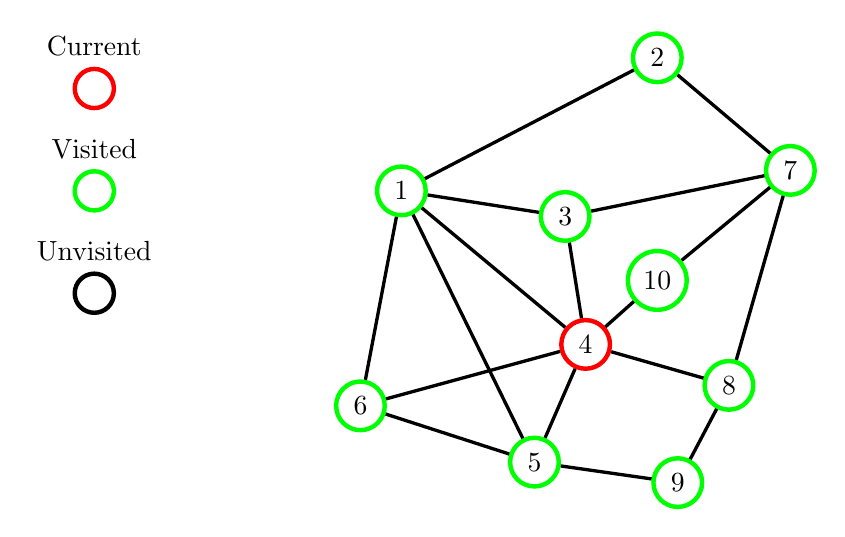
\begin{tikzpicture}[scale=1.3] 
\node[shape=circle, draw=red, 	ultra thick, scale=1.5pt, label={Current}] (U) at (-3, 1) {}; 
\node[shape=circle, draw=green,  ultra thick, scale=1.5pt, label={Visited}] (U) at (-3, 0) {}; 
\node[shape=circle, draw=black, ultra thick, scale=1.5pt, label={Unvisited}] (U) at (-3, -1) {}; 
\node[shape=circle,draw=green, ultra thick] (1) at (0,0) {1}; 
\node[shape=circle,draw=green, ultra thick] (2) at (2.5,1.3) {2}; 
\node[shape=circle,draw=green, ultra thick] (3) at (1.6,-0.25) {3}; 
\node[shape=circle,draw=red, ultra thick] (4) at (1.8,-1.5) {4}; 
\node[shape=circle,draw=green, ultra thick] (5) at (1.3,-2.65) {5}; 
\node[shape=circle,draw=green, ultra thick] (6) at (-0.4,-2.1) {6}; 
\node[shape=circle,draw=green, ultra thick] (7) at (3.8,0.2) {7}; 
\node[shape=circle,draw=green, ultra thick] (8) at (3.2,-1.9) {8}; 
\node[shape=circle,draw=green, ultra thick] (9) at (2.7,-2.85) {9}; 
\node[shape=circle,draw=green, ultra thick] (10) at (2.5,-0.875) {10}; 
\path [-,very thick, draw=black] (2) edge  (1);
\path [-,very thick, draw=black] (3) edge  (1);
\path [-,very thick, draw=black] (4) edge  (1);
\path [-,very thick, draw=black] (5) edge  (1);
\path [-,very thick, draw=black] (6) edge  (1);
\path [-,very thick, draw=black] (7) edge  (2);
\path [-,very thick, draw=black] (7) edge  (3);
\path [-,very thick, draw=black] (4) edge  (3);
\path [-,very thick, draw=black] (5) edge  (4);
\path [-,very thick, draw=black] (6) edge  (4);
\path [-,very thick, draw=black] (8) edge  (4);
\path [-,very thick, draw=black] (10) edge  (4);
\path [-,very thick, draw=black] (6) edge  (5);
\path [-,very thick, draw=black] (9) edge  (5);
\path [-,very thick, draw=black] (8) edge  (7);
\path [-,very thick, draw=black] (10) edge  (7);
\path [-,very thick, draw=black] (9) edge  (8);
\end{tikzpicture} 
\end{figure} 
\end{frame} 
\begin{frame}{DFS : Example}
\begin{figure}
\center
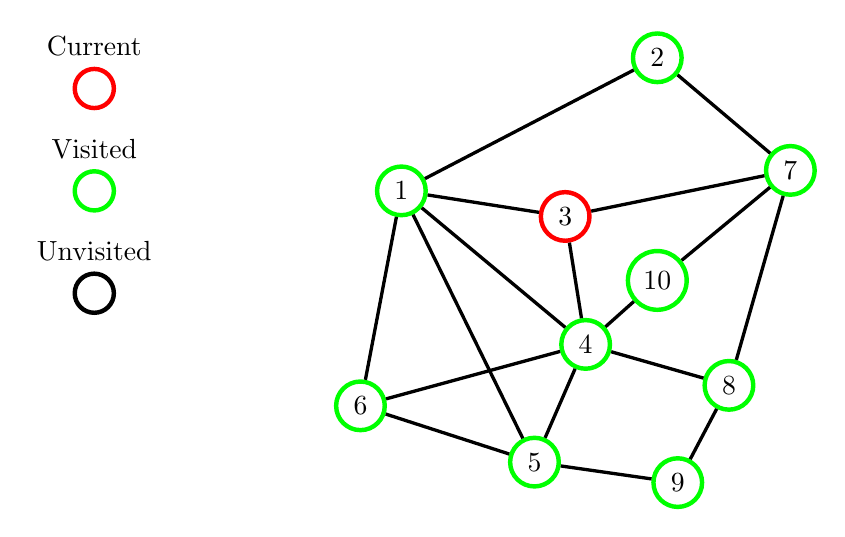
\begin{tikzpicture}[scale=1.3] 
\node[shape=circle, draw=red, 	ultra thick, scale=1.5pt, label={Current}] (U) at (-3, 1) {}; 
\node[shape=circle, draw=green,  ultra thick, scale=1.5pt, label={Visited}] (U) at (-3, 0) {}; 
\node[shape=circle, draw=black, ultra thick, scale=1.5pt, label={Unvisited}] (U) at (-3, -1) {}; 
\node[shape=circle,draw=green, ultra thick] (1) at (0,0) {1}; 
\node[shape=circle,draw=green, ultra thick] (2) at (2.5,1.3) {2}; 
\node[shape=circle,draw=red, ultra thick] (3) at (1.6,-0.25) {3}; 
\node[shape=circle,draw=green, ultra thick] (4) at (1.8,-1.5) {4}; 
\node[shape=circle,draw=green, ultra thick] (5) at (1.3,-2.65) {5}; 
\node[shape=circle,draw=green, ultra thick] (6) at (-0.4,-2.1) {6}; 
\node[shape=circle,draw=green, ultra thick] (7) at (3.8,0.2) {7}; 
\node[shape=circle,draw=green, ultra thick] (8) at (3.2,-1.9) {8}; 
\node[shape=circle,draw=green, ultra thick] (9) at (2.7,-2.85) {9}; 
\node[shape=circle,draw=green, ultra thick] (10) at (2.5,-0.875) {10}; 
\path [-,very thick, draw=black] (2) edge  (1);
\path [-,very thick, draw=black] (3) edge  (1);
\path [-,very thick, draw=black] (4) edge  (1);
\path [-,very thick, draw=black] (5) edge  (1);
\path [-,very thick, draw=black] (6) edge  (1);
\path [-,very thick, draw=black] (7) edge  (2);
\path [-,very thick, draw=black] (7) edge  (3);
\path [-,very thick, draw=black] (4) edge  (3);
\path [-,very thick, draw=black] (5) edge  (4);
\path [-,very thick, draw=black] (6) edge  (4);
\path [-,very thick, draw=black] (8) edge  (4);
\path [-,very thick, draw=black] (10) edge  (4);
\path [-,very thick, draw=black] (6) edge  (5);
\path [-,very thick, draw=black] (9) edge  (5);
\path [-,very thick, draw=black] (8) edge  (7);
\path [-,very thick, draw=black] (10) edge  (7);
\path [-,very thick, draw=black] (9) edge  (8);
\end{tikzpicture} 
\end{figure} 
\end{frame} 
\begin{frame}{DFS : Example}
\begin{figure}
\center
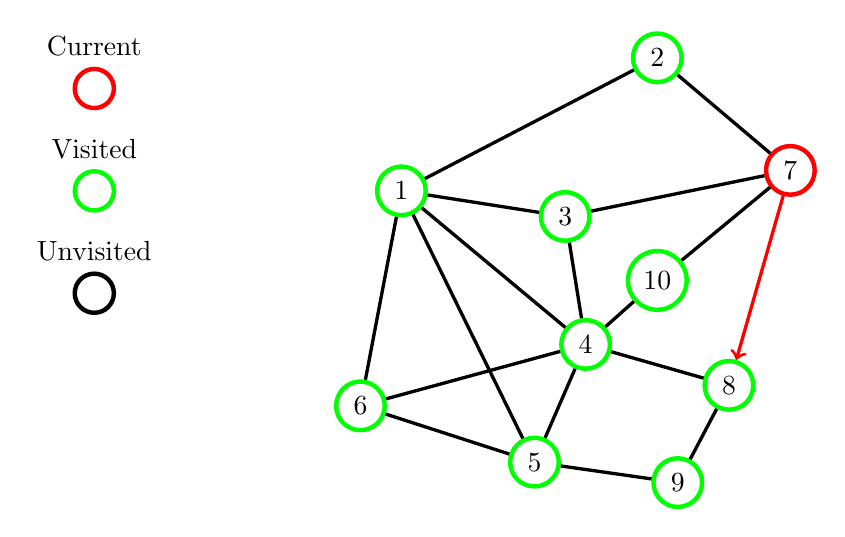
\begin{tikzpicture}[scale=1.3] 
\node[shape=circle, draw=red, 	ultra thick, scale=1.5pt, label={Current}] (U) at (-3, 1) {}; 
\node[shape=circle, draw=green,  ultra thick, scale=1.5pt, label={Visited}] (U) at (-3, 0) {}; 
\node[shape=circle, draw=black, ultra thick, scale=1.5pt, label={Unvisited}] (U) at (-3, -1) {}; 
\node[shape=circle,draw=green, ultra thick] (1) at (0,0) {1}; 
\node[shape=circle,draw=green, ultra thick] (2) at (2.5,1.3) {2}; 
\node[shape=circle,draw=green, ultra thick] (3) at (1.6,-0.25) {3}; 
\node[shape=circle,draw=green, ultra thick] (4) at (1.8,-1.5) {4}; 
\node[shape=circle,draw=green, ultra thick] (5) at (1.3,-2.65) {5}; 
\node[shape=circle,draw=green, ultra thick] (6) at (-0.4,-2.1) {6}; 
\node[shape=circle,draw=red, ultra thick] (7) at (3.8,0.2) {7}; 
\node[shape=circle,draw=green, ultra thick] (8) at (3.2,-1.9) {8}; 
\node[shape=circle,draw=green, ultra thick] (9) at (2.7,-2.85) {9}; 
\node[shape=circle,draw=green, ultra thick] (10) at (2.5,-0.875) {10}; 
\path [-,very thick, draw=black] (2) edge  (1);
\path [-,very thick, draw=black] (3) edge  (1);
\path [-,very thick, draw=black] (4) edge  (1);
\path [-,very thick, draw=black] (5) edge  (1);
\path [-,very thick, draw=black] (6) edge  (1);
\path [-,very thick, draw=black] (7) edge  (2);
\path [-,very thick, draw=black] (7) edge  (3);
\path [-,very thick, draw=black] (4) edge  (3);
\path [-,very thick, draw=black] (5) edge  (4);
\path [-,very thick, draw=black] (6) edge  (4);
\path [-,very thick, draw=black] (8) edge  (4);
\path [-,very thick, draw=black] (10) edge  (4);
\path [-,very thick, draw=black] (6) edge  (5);
\path [-,very thick, draw=black] (9) edge  (5);
\path [-,very thick, draw=black] (10) edge  (7);
\path [-,very thick, draw=black] (9) edge  (8);
\path [->,very thick, draw=red] (7) edge  (8);
\end{tikzpicture} 
\end{figure} 
\end{frame} 
\begin{frame}{DFS : Example}
\begin{figure}
\center
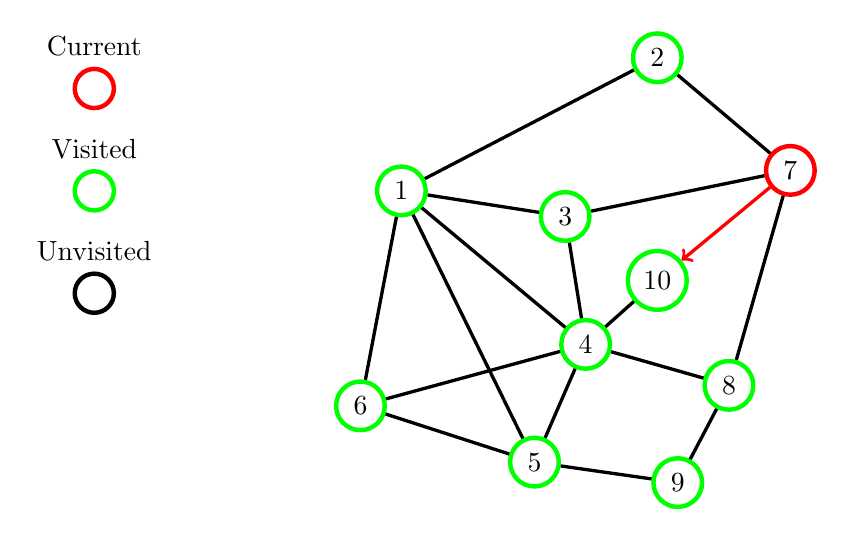
\begin{tikzpicture}[scale=1.3] 
\node[shape=circle, draw=red, 	ultra thick, scale=1.5pt, label={Current}] (U) at (-3, 1) {}; 
\node[shape=circle, draw=green,  ultra thick, scale=1.5pt, label={Visited}] (U) at (-3, 0) {}; 
\node[shape=circle, draw=black, ultra thick, scale=1.5pt, label={Unvisited}] (U) at (-3, -1) {}; 
\node[shape=circle,draw=green, ultra thick] (1) at (0,0) {1}; 
\node[shape=circle,draw=green, ultra thick] (2) at (2.5,1.3) {2}; 
\node[shape=circle,draw=green, ultra thick] (3) at (1.6,-0.25) {3}; 
\node[shape=circle,draw=green, ultra thick] (4) at (1.8,-1.5) {4}; 
\node[shape=circle,draw=green, ultra thick] (5) at (1.3,-2.65) {5}; 
\node[shape=circle,draw=green, ultra thick] (6) at (-0.4,-2.1) {6}; 
\node[shape=circle,draw=red, ultra thick] (7) at (3.8,0.2) {7}; 
\node[shape=circle,draw=green, ultra thick] (8) at (3.2,-1.9) {8}; 
\node[shape=circle,draw=green, ultra thick] (9) at (2.7,-2.85) {9}; 
\node[shape=circle,draw=green, ultra thick] (10) at (2.5,-0.875) {10}; 
\path [-,very thick, draw=black] (2) edge  (1);
\path [-,very thick, draw=black] (3) edge  (1);
\path [-,very thick, draw=black] (4) edge  (1);
\path [-,very thick, draw=black] (5) edge  (1);
\path [-,very thick, draw=black] (6) edge  (1);
\path [-,very thick, draw=black] (7) edge  (2);
\path [-,very thick, draw=black] (7) edge  (3);
\path [-,very thick, draw=black] (4) edge  (3);
\path [-,very thick, draw=black] (5) edge  (4);
\path [-,very thick, draw=black] (6) edge  (4);
\path [-,very thick, draw=black] (8) edge  (4);
\path [-,very thick, draw=black] (10) edge  (4);
\path [-,very thick, draw=black] (6) edge  (5);
\path [-,very thick, draw=black] (9) edge  (5);
\path [-,very thick, draw=black] (8) edge  (7);
\path [-,very thick, draw=black] (9) edge  (8);
\path [->,very thick, draw=red] (7) edge  (10);
\end{tikzpicture} 
\end{figure} 
\end{frame} 
\begin{frame}{DFS : Example}
\begin{figure}
\center
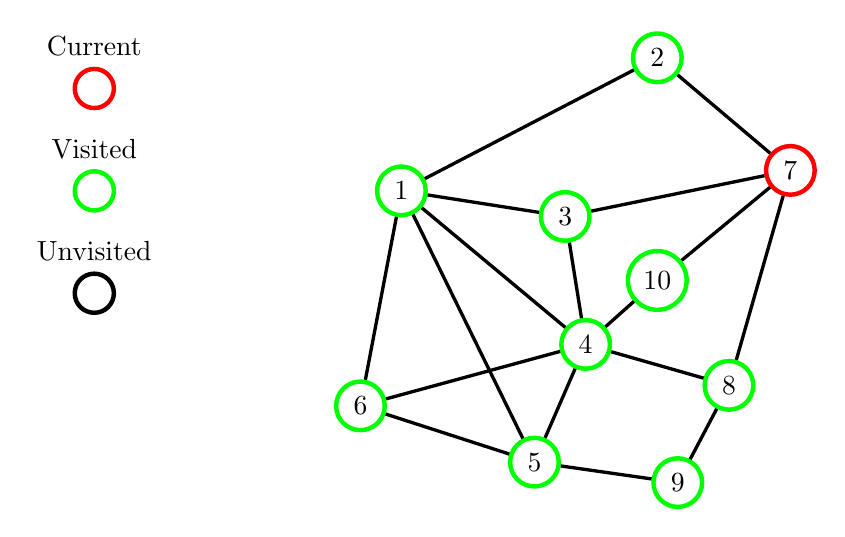
\begin{tikzpicture}[scale=1.3] 
\node[shape=circle, draw=red, 	ultra thick, scale=1.5pt, label={Current}] (U) at (-3, 1) {}; 
\node[shape=circle, draw=green,  ultra thick, scale=1.5pt, label={Visited}] (U) at (-3, 0) {}; 
\node[shape=circle, draw=black, ultra thick, scale=1.5pt, label={Unvisited}] (U) at (-3, -1) {}; 
\node[shape=circle,draw=green, ultra thick] (1) at (0,0) {1}; 
\node[shape=circle,draw=green, ultra thick] (2) at (2.5,1.3) {2}; 
\node[shape=circle,draw=green, ultra thick] (3) at (1.6,-0.25) {3}; 
\node[shape=circle,draw=green, ultra thick] (4) at (1.8,-1.5) {4}; 
\node[shape=circle,draw=green, ultra thick] (5) at (1.3,-2.65) {5}; 
\node[shape=circle,draw=green, ultra thick] (6) at (-0.4,-2.1) {6}; 
\node[shape=circle,draw=red, ultra thick] (7) at (3.8,0.2) {7}; 
\node[shape=circle,draw=green, ultra thick] (8) at (3.2,-1.9) {8}; 
\node[shape=circle,draw=green, ultra thick] (9) at (2.7,-2.85) {9}; 
\node[shape=circle,draw=green, ultra thick] (10) at (2.5,-0.875) {10}; 
\path [-,very thick, draw=black] (2) edge  (1);
\path [-,very thick, draw=black] (3) edge  (1);
\path [-,very thick, draw=black] (4) edge  (1);
\path [-,very thick, draw=black] (5) edge  (1);
\path [-,very thick, draw=black] (6) edge  (1);
\path [-,very thick, draw=black] (7) edge  (2);
\path [-,very thick, draw=black] (7) edge  (3);
\path [-,very thick, draw=black] (4) edge  (3);
\path [-,very thick, draw=black] (5) edge  (4);
\path [-,very thick, draw=black] (6) edge  (4);
\path [-,very thick, draw=black] (8) edge  (4);
\path [-,very thick, draw=black] (10) edge  (4);
\path [-,very thick, draw=black] (6) edge  (5);
\path [-,very thick, draw=black] (9) edge  (5);
\path [-,very thick, draw=black] (8) edge  (7);
\path [-,very thick, draw=black] (10) edge  (7);
\path [-,very thick, draw=black] (9) edge  (8);
\end{tikzpicture} 
\end{figure} 
\end{frame} 
\begin{frame}{DFS : Example}
\begin{figure}
\center
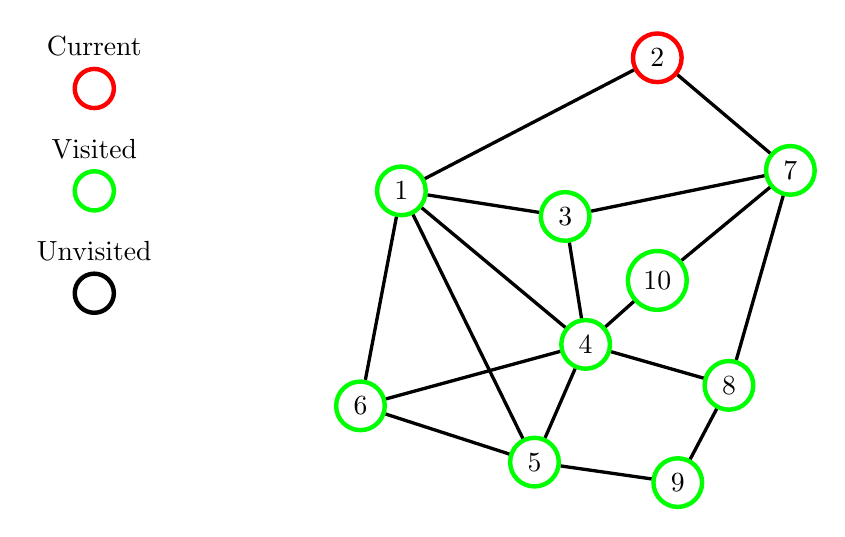
\begin{tikzpicture}[scale=1.3] 
\node[shape=circle, draw=red, 	ultra thick, scale=1.5pt, label={Current}] (U) at (-3, 1) {}; 
\node[shape=circle, draw=green,  ultra thick, scale=1.5pt, label={Visited}] (U) at (-3, 0) {}; 
\node[shape=circle, draw=black, ultra thick, scale=1.5pt, label={Unvisited}] (U) at (-3, -1) {}; 
\node[shape=circle,draw=green, ultra thick] (1) at (0,0) {1}; 
\node[shape=circle,draw=red, ultra thick] (2) at (2.5,1.3) {2}; 
\node[shape=circle,draw=green, ultra thick] (3) at (1.6,-0.25) {3}; 
\node[shape=circle,draw=green, ultra thick] (4) at (1.8,-1.5) {4}; 
\node[shape=circle,draw=green, ultra thick] (5) at (1.3,-2.65) {5}; 
\node[shape=circle,draw=green, ultra thick] (6) at (-0.4,-2.1) {6}; 
\node[shape=circle,draw=green, ultra thick] (7) at (3.8,0.2) {7}; 
\node[shape=circle,draw=green, ultra thick] (8) at (3.2,-1.9) {8}; 
\node[shape=circle,draw=green, ultra thick] (9) at (2.7,-2.85) {9}; 
\node[shape=circle,draw=green, ultra thick] (10) at (2.5,-0.875) {10}; 
\path [-,very thick, draw=black] (2) edge  (1);
\path [-,very thick, draw=black] (3) edge  (1);
\path [-,very thick, draw=black] (4) edge  (1);
\path [-,very thick, draw=black] (5) edge  (1);
\path [-,very thick, draw=black] (6) edge  (1);
\path [-,very thick, draw=black] (7) edge  (2);
\path [-,very thick, draw=black] (7) edge  (3);
\path [-,very thick, draw=black] (4) edge  (3);
\path [-,very thick, draw=black] (5) edge  (4);
\path [-,very thick, draw=black] (6) edge  (4);
\path [-,very thick, draw=black] (8) edge  (4);
\path [-,very thick, draw=black] (10) edge  (4);
\path [-,very thick, draw=black] (6) edge  (5);
\path [-,very thick, draw=black] (9) edge  (5);
\path [-,very thick, draw=black] (8) edge  (7);
\path [-,very thick, draw=black] (10) edge  (7);
\path [-,very thick, draw=black] (9) edge  (8);
\end{tikzpicture} 
\end{figure} 
\end{frame} 
\begin{frame}{DFS : Example}
\begin{figure}
\center
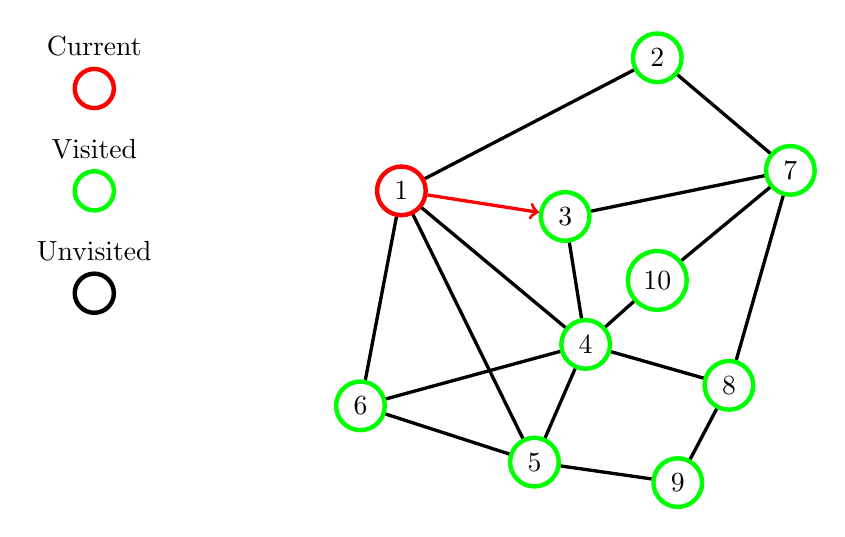
\begin{tikzpicture}[scale=1.3] 
\node[shape=circle, draw=red, 	ultra thick, scale=1.5pt, label={Current}] (U) at (-3, 1) {}; 
\node[shape=circle, draw=green,  ultra thick, scale=1.5pt, label={Visited}] (U) at (-3, 0) {}; 
\node[shape=circle, draw=black, ultra thick, scale=1.5pt, label={Unvisited}] (U) at (-3, -1) {}; 
\node[shape=circle,draw=red, ultra thick] (1) at (0,0) {1}; 
\node[shape=circle,draw=green, ultra thick] (2) at (2.5,1.3) {2}; 
\node[shape=circle,draw=green, ultra thick] (3) at (1.6,-0.25) {3}; 
\node[shape=circle,draw=green, ultra thick] (4) at (1.8,-1.5) {4}; 
\node[shape=circle,draw=green, ultra thick] (5) at (1.3,-2.65) {5}; 
\node[shape=circle,draw=green, ultra thick] (6) at (-0.4,-2.1) {6}; 
\node[shape=circle,draw=green, ultra thick] (7) at (3.8,0.2) {7}; 
\node[shape=circle,draw=green, ultra thick] (8) at (3.2,-1.9) {8}; 
\node[shape=circle,draw=green, ultra thick] (9) at (2.7,-2.85) {9}; 
\node[shape=circle,draw=green, ultra thick] (10) at (2.5,-0.875) {10}; 
\path [-,very thick, draw=black] (2) edge  (1);
\path [-,very thick, draw=black] (4) edge  (1);
\path [-,very thick, draw=black] (5) edge  (1);
\path [-,very thick, draw=black] (6) edge  (1);
\path [-,very thick, draw=black] (7) edge  (2);
\path [-,very thick, draw=black] (7) edge  (3);
\path [-,very thick, draw=black] (4) edge  (3);
\path [-,very thick, draw=black] (5) edge  (4);
\path [-,very thick, draw=black] (6) edge  (4);
\path [-,very thick, draw=black] (8) edge  (4);
\path [-,very thick, draw=black] (10) edge  (4);
\path [-,very thick, draw=black] (6) edge  (5);
\path [-,very thick, draw=black] (9) edge  (5);
\path [-,very thick, draw=black] (8) edge  (7);
\path [-,very thick, draw=black] (10) edge  (7);
\path [-,very thick, draw=black] (9) edge  (8);
\path [->,very thick, draw=red] (1) edge  (3);
\end{tikzpicture} 
\end{figure} 
\end{frame} 
\begin{frame}{DFS : Example}
\begin{figure}
\center
\begin{tikzpicture}[scale=1.3] 
\node[shape=circle, draw=red, 	ultra thick, scale=1.5pt, label={Current}] (U) at (-3, 1) {}; 
\node[shape=circle, draw=green,  ultra thick, scale=1.5pt, label={Visited}] (U) at (-3, 0) {}; 
\node[shape=circle, draw=black, ultra thick, scale=1.5pt, label={Unvisited}] (U) at (-3, -1) {}; 
\node[shape=circle,draw=red, ultra thick] (1) at (0,0) {1}; 
\node[shape=circle,draw=green, ultra thick] (2) at (2.5,1.3) {2}; 
\node[shape=circle,draw=green, ultra thick] (3) at (1.6,-0.25) {3}; 
\node[shape=circle,draw=green, ultra thick] (4) at (1.8,-1.5) {4}; 
\node[shape=circle,draw=green, ultra thick] (5) at (1.3,-2.65) {5}; 
\node[shape=circle,draw=green, ultra thick] (6) at (-0.4,-2.1) {6}; 
\node[shape=circle,draw=green, ultra thick] (7) at (3.8,0.2) {7}; 
\node[shape=circle,draw=green, ultra thick] (8) at (3.2,-1.9) {8}; 
\node[shape=circle,draw=green, ultra thick] (9) at (2.7,-2.85) {9}; 
\node[shape=circle,draw=green, ultra thick] (10) at (2.5,-0.875) {10}; 
\path [-,very thick, draw=black] (2) edge  (1);
\path [-,very thick, draw=black] (3) edge  (1);
\path [-,very thick, draw=black] (5) edge  (1);
\path [-,very thick, draw=black] (6) edge  (1);
\path [-,very thick, draw=black] (7) edge  (2);
\path [-,very thick, draw=black] (7) edge  (3);
\path [-,very thick, draw=black] (4) edge  (3);
\path [-,very thick, draw=black] (5) edge  (4);
\path [-,very thick, draw=black] (6) edge  (4);
\path [-,very thick, draw=black] (8) edge  (4);
\path [-,very thick, draw=black] (10) edge  (4);
\path [-,very thick, draw=black] (6) edge  (5);
\path [-,very thick, draw=black] (9) edge  (5);
\path [-,very thick, draw=black] (8) edge  (7);
\path [-,very thick, draw=black] (10) edge  (7);
\path [-,very thick, draw=black] (9) edge  (8);
\path [->,very thick, draw=red] (1) edge  (4);
\end{tikzpicture} 
\end{figure} 
\end{frame} 
\begin{frame}{DFS : Example}
\begin{figure}
\center
\begin{tikzpicture}[scale=1.3] 
\node[shape=circle, draw=red, 	ultra thick, scale=1.5pt, label={Current}] (U) at (-3, 1) {}; 
\node[shape=circle, draw=green,  ultra thick, scale=1.5pt, label={Visited}] (U) at (-3, 0) {}; 
\node[shape=circle, draw=black, ultra thick, scale=1.5pt, label={Unvisited}] (U) at (-3, -1) {}; 
\node[shape=circle,draw=red, ultra thick] (1) at (0,0) {1}; 
\node[shape=circle,draw=green, ultra thick] (2) at (2.5,1.3) {2}; 
\node[shape=circle,draw=green, ultra thick] (3) at (1.6,-0.25) {3}; 
\node[shape=circle,draw=green, ultra thick] (4) at (1.8,-1.5) {4}; 
\node[shape=circle,draw=green, ultra thick] (5) at (1.3,-2.65) {5}; 
\node[shape=circle,draw=green, ultra thick] (6) at (-0.4,-2.1) {6}; 
\node[shape=circle,draw=green, ultra thick] (7) at (3.8,0.2) {7}; 
\node[shape=circle,draw=green, ultra thick] (8) at (3.2,-1.9) {8}; 
\node[shape=circle,draw=green, ultra thick] (9) at (2.7,-2.85) {9}; 
\node[shape=circle,draw=green, ultra thick] (10) at (2.5,-0.875) {10}; 
\path [-,very thick, draw=black] (2) edge  (1);
\path [-,very thick, draw=black] (3) edge  (1);
\path [-,very thick, draw=black] (4) edge  (1);
\path [-,very thick, draw=black] (6) edge  (1);
\path [-,very thick, draw=black] (7) edge  (2);
\path [-,very thick, draw=black] (7) edge  (3);
\path [-,very thick, draw=black] (4) edge  (3);
\path [-,very thick, draw=black] (5) edge  (4);
\path [-,very thick, draw=black] (6) edge  (4);
\path [-,very thick, draw=black] (8) edge  (4);
\path [-,very thick, draw=black] (10) edge  (4);
\path [-,very thick, draw=black] (6) edge  (5);
\path [-,very thick, draw=black] (9) edge  (5);
\path [-,very thick, draw=black] (8) edge  (7);
\path [-,very thick, draw=black] (10) edge  (7);
\path [-,very thick, draw=black] (9) edge  (8);
\path [->,very thick, draw=red] (1) edge  (5);
\end{tikzpicture} 
\end{figure} 
\end{frame} 
\begin{frame}{DFS : Example}
\begin{figure}
\center
\begin{tikzpicture}[scale=1.3] 
\node[shape=circle, draw=red, 	ultra thick, scale=1.5pt, label={Current}] (U) at (-3, 1) {}; 
\node[shape=circle, draw=green,  ultra thick, scale=1.5pt, label={Visited}] (U) at (-3, 0) {}; 
\node[shape=circle, draw=black, ultra thick, scale=1.5pt, label={Unvisited}] (U) at (-3, -1) {}; 
\node[shape=circle,draw=red, ultra thick] (1) at (0,0) {1}; 
\node[shape=circle,draw=green, ultra thick] (2) at (2.5,1.3) {2}; 
\node[shape=circle,draw=green, ultra thick] (3) at (1.6,-0.25) {3}; 
\node[shape=circle,draw=green, ultra thick] (4) at (1.8,-1.5) {4}; 
\node[shape=circle,draw=green, ultra thick] (5) at (1.3,-2.65) {5}; 
\node[shape=circle,draw=green, ultra thick] (6) at (-0.4,-2.1) {6}; 
\node[shape=circle,draw=green, ultra thick] (7) at (3.8,0.2) {7}; 
\node[shape=circle,draw=green, ultra thick] (8) at (3.2,-1.9) {8}; 
\node[shape=circle,draw=green, ultra thick] (9) at (2.7,-2.85) {9}; 
\node[shape=circle,draw=green, ultra thick] (10) at (2.5,-0.875) {10}; 
\path [-,very thick, draw=black] (2) edge  (1);
\path [-,very thick, draw=black] (3) edge  (1);
\path [-,very thick, draw=black] (4) edge  (1);
\path [-,very thick, draw=black] (5) edge  (1);
\path [-,very thick, draw=black] (7) edge  (2);
\path [-,very thick, draw=black] (7) edge  (3);
\path [-,very thick, draw=black] (4) edge  (3);
\path [-,very thick, draw=black] (5) edge  (4);
\path [-,very thick, draw=black] (6) edge  (4);
\path [-,very thick, draw=black] (8) edge  (4);
\path [-,very thick, draw=black] (10) edge  (4);
\path [-,very thick, draw=black] (6) edge  (5);
\path [-,very thick, draw=black] (9) edge  (5);
\path [-,very thick, draw=black] (8) edge  (7);
\path [-,very thick, draw=black] (10) edge  (7);
\path [-,very thick, draw=black] (9) edge  (8);
\path [->,very thick, draw=red] (1) edge  (6);
\end{tikzpicture} 
\end{figure} 
\end{frame} 
\begin{frame}{DFS : Example}
\begin{figure}
\center
\begin{tikzpicture}[scale=1.3] 
\node[shape=circle, draw=red, 	ultra thick, scale=1.5pt, label={Current}] (U) at (-3, 1) {}; 
\node[shape=circle, draw=green,  ultra thick, scale=1.5pt, label={Visited}] (U) at (-3, 0) {}; 
\node[shape=circle, draw=black, ultra thick, scale=1.5pt, label={Unvisited}] (U) at (-3, -1) {}; 
\node[shape=circle,draw=red, ultra thick] (1) at (0,0) {1}; 
\node[shape=circle,draw=green, ultra thick] (2) at (2.5,1.3) {2}; 
\node[shape=circle,draw=green, ultra thick] (3) at (1.6,-0.25) {3}; 
\node[shape=circle,draw=green, ultra thick] (4) at (1.8,-1.5) {4}; 
\node[shape=circle,draw=green, ultra thick] (5) at (1.3,-2.65) {5}; 
\node[shape=circle,draw=green, ultra thick] (6) at (-0.4,-2.1) {6}; 
\node[shape=circle,draw=green, ultra thick] (7) at (3.8,0.2) {7}; 
\node[shape=circle,draw=green, ultra thick] (8) at (3.2,-1.9) {8}; 
\node[shape=circle,draw=green, ultra thick] (9) at (2.7,-2.85) {9}; 
\node[shape=circle,draw=green, ultra thick] (10) at (2.5,-0.875) {10}; 
\path [-,very thick, draw=black] (2) edge  (1);
\path [-,very thick, draw=black] (3) edge  (1);
\path [-,very thick, draw=black] (4) edge  (1);
\path [-,very thick, draw=black] (5) edge  (1);
\path [-,very thick, draw=black] (6) edge  (1);
\path [-,very thick, draw=black] (7) edge  (2);
\path [-,very thick, draw=black] (7) edge  (3);
\path [-,very thick, draw=black] (4) edge  (3);
\path [-,very thick, draw=black] (5) edge  (4);
\path [-,very thick, draw=black] (6) edge  (4);
\path [-,very thick, draw=black] (8) edge  (4);
\path [-,very thick, draw=black] (10) edge  (4);
\path [-,very thick, draw=black] (6) edge  (5);
\path [-,very thick, draw=black] (9) edge  (5);
\path [-,very thick, draw=black] (8) edge  (7);
\path [-,very thick, draw=black] (10) edge  (7);
\path [-,very thick, draw=black] (9) edge  (8);
\end{tikzpicture} 
\end{figure} 
\end{frame} 
